
\documentclass[preprint,12pt,3p]{elsarticle}


\usepackage{amssymb}
\usepackage{amsmath}
\usepackage{yhmath}
\usepackage{amsthm}
\usepackage{url}
\usepackage{comment}
\usepackage{xcolor}
\usepackage{bigints}
\allowdisplaybreaks



\newtheorem{thm}{Theorem}
\newdefinition{lem}{Lemma}
\newdefinition{rmk}{Remark}
\newdefinition{definition}{Definition}
\newdefinition{cor}{Corollary}
\newproof{pf}{Proof}
\newcommand{\dd}{ {\rm d} }

\newcommand{\pv}{\operatorname{p.\!v.}}

\newcommand{\bx}{{\mathbf{x}}}
\newcommand{\by}{{\mathbf{y}}}
\newcommand{\br}{{\mathbf{r}}}

\DeclareMathOperator{\sign}{sign}

\journal{.}

\begin{document}

\begin{frontmatter}



\title{Boundary Integral Formulations for Flexural Wave Scattering in Thin Plates}



\affiliation[1]{organization={Committee on Computational and Applied Mathematics, University of Chicago},
addressline={5747 S. Ellis Avenue},
postcode={60637},
city={Chicago, IL},
country={USA}}

\affiliation[2]{organization={Department of Mathematical Sciences, New Jersey Institute of Technology},
addressline={Cullimore Hall},
postcode={07102},
city={Newark, NJ},
country={USA}}

\author[1]{Peter Nekrasov\corref{cor1}}
\ead{pn3@uchicago.edu}

\author[1]{Tim Su}

\author[2]{Travis Askham}
 
\author[1]{Jeremy G. Hoskins}


\cortext[cor1]{Corresponding author.  }


\begin{abstract}
In this paper we develop second kind integral formulations  for flexural wave scattering problems involving the clamped, free, and supported plate boundary conditions. While the clamped plate problem can be solved with layer potentials previously developed for the biharmonic equation \cite{farkas}, the free plate problem is more difficult due to the complex nature of the boundary conditions. In this paper we describe a representation for the free plate problem that uses the Hilbert transform to cancel singularities of certain layer potentials, ultimately leading to a Fredholm integral equation of the second kind. Additionally, for the supported plate problem, we improve on an existing representation to obtain a second kind integral equation.  With these representations, it is possible to solve flexural wave scattering problems with high-order-accurate methods, examine the far-field patterns of scattering objects, and solve large problems involving multiple scatterers.
\end{abstract}



\begin{keyword}
Integral equations \sep biharmonic \sep elasticity \sep Hilbert transform \sep fast algorithms

\end{keyword}

\end{frontmatter}


\section{Background}

Scientific interest in the vibrations of free plates can be traced as far back as Ernst Chladni's famous demonstration in front of Napoleon at the Paris Academy in 1808. In the century that followed, the theory of plates developed rapidly through the work of Kirchhoff \cite{Kirchhoff1850} and Love \cite{love} and was later refined and popularized by Timoshenko \cite{timoshenko1959theory}. Today, this theory is applied to the modeling and observation of elastic waves in many engineering and geophysics contexts. These vibrations, known as flexural waves, were responsible for bringing down the Tacoma Narrows Bridge \cite{Drabek2003}, while the same vibrations led to substantial calving in the Larsen A and B and Wilkins ice shelves \cite{massom18}. In short, flexural phenomena pose a significant challenge to the integrity of both the natural and built environments. 

Flexural waves are typically modelled by the thin plate approximation, where the vertical displacement of a plate is defined as a scalar function of two horizontal dimensions. For some closed subset of the plane $\Omega \subset \mathbb{R}^2$ and $\mathbf{x}:=(x,y) \in \Omega$, the out-of-plane displacement $u(\mathbf{x})$ is described by the following fourth-order partial differential equation (PDE):
\begin{align}
    \Delta^2 u - k^4 u = 0 \qquad \text{ on } \Omega \label{flexural}
\end{align}
where $\Delta^2 u := \displaystyle \frac{\partial^4 u }{\partial x^4} + 2 \frac{\partial^4 u}{\partial x^2 \partial y^2} + \frac{\partial^4 u}{\partial y^4}$ is the biharmonic operator and $k$ is the wavenumber. The first term in the equation corresponds to a bending force, while the second term represents the inertia after assuming that the solution is harmonic in time. Equation \eqref{flexural} can also be thought of as an eigenvalue problem corresponding to the biharmonic operator.

Since equation \eqref{flexural} is fourth-order, two boundary conditions (BCs) are required to fully determine the problem. In the present work, we are concerned with the three sets of boundary conditions that arise most frequently in thin plate theory: the clamped, free, and supported plates \cite{timoshenko1959theory, ritz09, Friedrichs1928,kato1957estimation, landau59}. The clamped plate BCs restrict the motion of the plate at the boundary by fixing both the displacement and slope, while the free plate BCs prescribe bending and shear forces, allowing the displacement and slope to oscillate at the boundary. Lastly, the supported plate restricts displacement but allows for sloping, leading to a combination of fixed and flexible behavior. The precise description for these boundary conditions, as well as examples of where they arise, are given in Sections \ref{clampedsection}, \ref{freesection}, and \ref{supportedsection}. 

There are many physical reasons to study exterior problems involving these boundary conditions. Plates that are found in buildings and bridges may be supported from within by internal columns, rods, and springs that affect their flexure \cite{zhao2002plate}. Alternatively, cut-outs can also made to these plates to lighten or ventilate the structure \cite{RAJAMANI1977549, HUANG1999769}. These inclusions are often used to alter or eliminate resonant modes \cite{PhysRevB.73.064301, Lindsay2018}. This is valuable in the field of acoustics, where one is typically searching for a very specific frequency response \cite{ ZHU2024108814, laulagnet1998sound}. While the majority of our focus in this paper is on exterior problems, the techniques outlined here can also be applied for studying interior problems.

Traditionally, interior problems involving these boundary conditions have been treated using the finite element method (FEM) \cite{ monk87, climente2014gradient, mora2009piecewise, meylan2002}. For the clamped and supported plate problems, there are well-understood error estimates \cite{ishihara78, BRAMBLE1983} and software packages available for dealing with complex geometries. However, very few error estimates or high-order implementations exist for the free plate problem, which is typically solved on relatively simple geometries. FEM also makes it challenging to study exterior problems since it requires one to discretize the entire region containing both the scattering object and the points where one hopes to obtain the solution, while truncating the domain and solving auxiliary constraints at artificial boundaries.  This is either done with transparent boundary conditions \cite{YUE2023100350, YUE2024112606} or perfectly matched layers \cite{FARHAT20112237}, where it is difficult to achieve zero reflectance for complicated wave phenomena. 

An alternative approach is to recast the PDE as an integral equation defined on the boundary of the domain. 
In general, this is possible whenever the PDE is linear and elliptic, with known Green's function \cite{Atkinson_1997}. 
The basic approach is to define the solution of the PDE in terms of a layer potential with an unknown density
defined on the boundary of the domain. The layer potential is designed to automatically 
satisfy the PDE within the domain, while the unknown density is determined by enforcing the boundary conditions on the
boundary traces of the layer potential, resulting in a boundary integral equation (BIE).

Numerically, BIEs offer several advantages over direct discretization or weak formulation of the
PDE. One feature of BIEs is that all of the unknowns are located on the boundary of the domain, and hence only the boundary needs to be discretized. This is particularly useful for solving exterior problems, where any necessary 
radiation conditions can be incorporated into the definition of the layer potential. There are further 
advantages for BIEs that are also second kind integral equations (SKIEs) in which the operator applied to the density is the sum 
of a bounded invertible operator and a compact operator. There is a well-established theory for analyzing the 
existence and uniqueness of solutions to SKIEs via the Fredholm alternative, as well as their behavior 
under discretization~\cite{kress,colton2013integral,Hackbusch1995}. In particular, the condition number of the discretized SKIE system will remain bounded as 
the boundary mesh is refined. 

There is a significant literature for BIEs in the biharmonic problem ($k=0$),
particularly for the clamped plate boundary conditions. SKIEs based on multiple-layer representations
were historically applied to analyze the existence, uniqueness, and regularity of solutions of the clamped plate 
problem~\cite{agmon1957multiple,cohen1983dirichlet}. An alternative route to the clamped plate problem
can be pursued by converting the problem to a Stokes problem, for which there are particularly
nice representations~\cite{muschelivsvili1933research,Rachh2018}.
A general approach for the $k=0$ case with both clamped plate and free plate BCs
is developed in~\cite[\S 2.4]{hsiao2008boundary} by analogy with the second order
case, though the resulting boundary operators are not exactly SKIEs but include hypersingular operators. 
It is also possible to solve the supported plate problem by reduction
to a system of two Poisson equations  \cite{parisdeleon, sladek}, but this method requires volume integration and has no clear extension to the case when $k \neq 0$.

The thesis~\cite{farkas} describes a different framework for developing layer potential representations. The
basic idea is to select linear combinations of derivatives of the Green's function such that the 
resulting BIE is second kind and that the integral kernels in the BIE are as smooth as possible. In~\cite{farkas},
the technique is applied to the $k=0$ case for the clamped plate, fluid mechanics ($\nabla u$ is prescribed on the boundary),
and supported plate BCs,
though with limited success in the case of the fluid mechanics and supported plate BCs. 
In particular, the BIEs for the fluid mechanics and supported plate problems contain differential operators and therefore their condition number is unbounded. For the clamped plate problem, the framework of~\cite{farkas} extends readily
to three dimensions~\cite{JIANG20117488} and to nonzero $k$~\cite{Lindsay2018}.

In contrast with the steady-state ($k=0$) case, the oscillatory problem has received less attention, 
despite being a central focus of texts on structural engineering and elastic 
physics~\cite{timoshenko1959theory, landau59}. Previous attempts have relied on factoring the solution 
into Helmholtz and modified Helmholtz equations and solving a coupled system at the 
boundary~\cite{YUE2023100350, Dong2024, SMITH20114029}. 
These combined BIEs can suffer from ill-conditioning
though effective pre-conditioning strategies exist~\cite{Dong2024}. These approaches are currently not capable of solving the free or supported plate problems, which motivates the development of the present BIEs. Compared with previous methods, we gain degrees of freedom in the design of the integral representation by taking standard layer potentials and composing them with the Hilbert transform. 


The remainder of the paper is as follows. In section \ref{biesection}, we give an overview of the Green's function and the boundary integral framework that will be used to solve this problem. In section~\ref{clampedsection}, we review
the kernels previously used by~\cite{farkas, Lindsay2018} for solving the clamped plate problem and discuss their application to exterior 
problems. In section~\ref{freesection}, we present a novel representation for the free plate problem which uses the Hilbert transform in the representation of the solution. In section~\ref{supportedsection}, we give a representation for the supported plate which is similar to~\cite{farkas}, but uses extra terms to ensure that the BIE is second kind. In section~\ref{num_imp}, we discuss details of the implementation of these methods used for the
numerical results, describing a high-order-accurate approach to discretize the integral equations and stable methods to evaluate the kernels. In section~\ref{results}, we present numerical results illustrating high-order convergence, and the application of these methods to solve scattering problems, including scattering from a large collection of objects. Finally, in section~\ref{discussion}, we discuss the significance of the present work and the potential for using integral equations to model sea ice and ice shelves in the future. 

\section{Mathematical Framework and BIE Formalism} \label{biesection}

The Green's function for the free-space problem is defined as the solution to the equation
\begin{align}
    \Delta^2 u - k^4 u = \delta(\mathbf{x} - \mathbf{y})
\end{align}
where $\mathbf{x},\mathbf{y} \in  \mathbb{R}^2$, supplemented with the following radiation condition at infinity:
\begin{equation}
\label{eq:radcond}
   \frac{\bx}{|\bx|} \cdot \nabla u - i k u = o(1/\sqrt{|\bx|}) \; . 
\end{equation}
The Green's function for this problem can be written explicitly as 
\begin{align}
    G(\mathbf{x},\mathbf{y}) &=  \frac{1}{2k^2} \left[ \frac{i}{4} H_0^{(1)} (k |\mathbf{x} - \mathbf{y}|) - \frac{1}{2\pi} K_0 (k | \mathbf{x} - \mathbf{y}|) \right] \label{greens} 
\end{align}
 where $H_0^{(1)}$ is the zero-th order Hankel function of the first kind and $K_0$ is the zero-th order modified Bessel function of the second kind. 
 This Green's function is a scaled difference of the Green's functions for the Helmholtz and Yukawa equations, which oscillate and decay, respectively. As such, $G$ automatically satisfies the natural radiation condition \eqref{eq:radcond}.

In the BIE framework, we seek to represent the solution to a boundary value problem (BVP) as a combination of integral operators applied to some densities on the boundary:
\begin{align}
\label{eq:layerpotential}
    u(\mathbf{x}) &= \mathcal{K}_1 [\rho_1 ](\mathbf{x}) + \mathcal{K}_2 [\rho_2 ](\mathbf{x}) 
\end{align}
where $\rho_1 $ and $\rho_2 $ are densities that lie in a suitable function space on the 
boundary (e.g. $L^2(\partial \Omega)$) and where the integral operators $\mathcal{K}_1$ and $\mathcal{K}_2$ are given by
\begin{align}
    \mathcal{K}_1[\rho_1](\mathbf{x}) &:= \int_{\partial \Omega} K_1(\mathbf{x},\mathbf{y}) \rho_1(\mathbf{y})  \, \dd S(\mathbf{y})  \\
    \mathcal{K}_2[\rho_2](\mathbf{x}) &:= \int_{\partial \Omega} K_2(\mathbf{x},\mathbf{y}) \rho_2(\mathbf{y})  \, \dd S(\mathbf{y})  \; .
\end{align}

In this formalism, we represent the solution of the BVP using a collection of ``charges'' (sources, dipoles, and multipoles) defined on the boundary $\partial\Omega$. The kernels $K_1$ and $K_2$ typically involve derivatives of the Green's function, so that the representation automatically satisfies \eqref{flexural} in the interior. To ensure that this solution also satisfies the BCs, one must plug this representation into the boundary conditions and take the limit as the target approaches the boundary. This leads to a $2\times 2$ system of integral  equations on the boundary $\partial \Omega$:
\begin{equation}
\label{eq:biesystem}
    \begin{pmatrix}
    D_{11} & D_{12} \\
    D_{21} & D_{22}
    \end{pmatrix}
    \begin{pmatrix}
        \rho_1(\mathbf{x}) \\
        \rho_2(\mathbf{x}) 
    \end{pmatrix} + \pv \int_{\partial \Omega} \begin{pmatrix}
    K_{11}(\mathbf{x},\mathbf{y}) & K_{12}(\mathbf{x},\mathbf{y}) \\
    K_{21}(\mathbf{x},\mathbf{y}) & K_{22}(\mathbf{x},\mathbf{y})
    \end{pmatrix}
    \begin{pmatrix}
        \rho_1(\mathbf{y}) \\
        \rho_2(\mathbf{y})
    \end{pmatrix} \, \dd S(\mathbf{y})
    = \begin{pmatrix}
        f_1(\mathbf{x}) \\ f_2(\mathbf{x})
    \end{pmatrix} \; ,
\end{equation}
where $\pv$ indicates that the (possibly singular) integral is to be understood in the principal
value sense. It is useful to define the on-surface integral operators as well:
\begin{align}
    \mathcal{K}_{ij}[\rho_j](\mathbf{x}) &:= \pv \int_{\partial \Omega} K_{ij}(\mathbf{x},\mathbf{y}) \rho_j(\mathbf{y})  \, \dd S(\mathbf{y}) 
\end{align}
The jump matrix $ \mathbf{D} := \begin{pmatrix}
    D_{11} & D_{12} \\
    D_{21} & D_{22}
    \end{pmatrix} $ is often referred to as the constant or identity part of the integral equation and is precisely the difference between the limit of the integral operator as it approaches the boundary and the operator on the boundary:
    \begin{align}
        D_{ij} \rho_j(\mathbf{x}_0) :=  \lim_{\mathbf{x} \rightarrow \mathbf{x}_0} \int_{\partial\Omega} K_{ij}(\mathbf{x},\mathbf{y}) \rho_j(\mathbf{y}) \, \dd S(\mathbf{y}) - \pv \int_{\partial\Omega} K_{ij}(\mathbf{x}_0,\mathbf{y}) \rho_j(\mathbf{y}) \, \dd S(\mathbf{y})
    \end{align}
    Meanwhile, the kernel matrix $\mathbf{K} := \begin{pmatrix}
    K_{11} & K_{12} \\
    K_{21} & K_{22}
    \end{pmatrix} $ consists of the kernels $K_1$ and $K_2$ plugged into the corresponding boundary conditions. The expressions $f_1$ and $f_2$ on the right-hand side depend on the boundary data. When the jump matrix $\mathbf{D}$ is bounded and invertible and the integral
    operators $\mathcal{K}_{ij}$ are compact, the equation is referred to as a second kind integral equation (SKIE). 
    The goal of this paper is to design kernels $K_1$ and $K_2$ for each of the clamped plate, free plate, and supported
    plate BCs so that system \eqref{eq:biesystem} is an SKIE. 
    
In the remainder of the manuscript, we use the following conventions for notation. 
The boundary, $\partial \Omega$, is assumed to be a smooth curve. 
For a point $\bx$ on $\partial \Omega$, $n(\bx)$ is the outward-pointing normal,
$\tau(\bx)$ is the positively-oriented (clockwise) unit tangent vector, and $\kappa(\bx)$ is 
the signed curvature at the point $\bx$. The value $s$ denotes arc-length along the curve. 
The input to the Green's function is usually of the form $G(\bx,\by)$, where $\bx$ is 
sometimes referred to as the ``target'' and $\by$ as the ``source.'' We often employ the 
more compact notation $n_\mathbf{x} = n(\bx)$, $\tau_\mathbf{y}=\tau(\by)$, etc. We denote directional derivatives of the Green's function by subscripts, e.g. 
$G_{n_\bx}(\bx,\by) = n(\bx) \cdot \nabla_\mathbf{x} G(\bx,\by)$ and $G_{\tau_\by} = \tau(\by) \cdot \nabla_\by G$. 
Multiple subscripts correspond to contractions of the Hessian or other higher-order
derivative tensors of $G$ with the indicated directions, e.g. 
\begin{equation}
    G_{n_\bx \tau_\bx \tau_\by}(\bx,\by) = n_\bx \cdot \nabla_\mathbf{w} \left ( \tau_\bx \cdot \nabla_\mathbf{w} \left ( \tau_\by \cdot \nabla_\mathbf{z} G(\mathbf{w},\mathbf{z})
    \right ) \right )  |_{\mathbf{w}=\bx,\mathbf{z}=\by} 
\end{equation}
An important distinction is that
\begin{equation}
\frac{\dd}{\dd s} G(\bx(s),\by) = G_{\tau_\bx}(\bx(s),\by) \quad \textrm{but} \quad 
\frac{\dd^2}{\dd s^2} G(\bx(s),\by) = G_{\tau_\bx \tau_\bx}(\bx(s),\by) -
\kappa(\bx(s)) G_{n_\bx}(\bx(s),\by)
\end{equation}
which can be easily seen through application of the product rule. 


\section{Clamped Plate Problem} \label{clampedsection}

First we consider the BVP with clamped plate BCs:
\begin{align}
    \begin{cases}
    \displaystyle u = f_1 \qquad &\text{ on } \partial \Omega  \\
    \displaystyle \frac{\partial u}{\partial n}  = f_2 \qquad &\text{ on } \partial \Omega 
    \end{cases} \label{clampedbcs}
\end{align}
These BCs are commonly used in engineering when a planar material is welded to its frame along the perimeter, such as the hull of a ship \cite{lakitosh2012analysis} or an aircraft wing \cite{kapania2000static, giles}. Within geophysics, these boundary conditions are used to describe floating ice that is anchored along its edges, for instance an ice shelf that is permanently moored at its grounding line \cite{sergienko13, Nekrasov_MacAyeal_2023}. When a plate is fixed at its boundary, it is unable to bend to absorb and release the energy of the wave. This creates a state of high internal stress near the grounding line of an ice shelf \cite{sergienko17}, making it a vulnerable and therefore important area to study \cite{FRIEDL2020102948}. 

As noted in the introduction, \cite{farkas} developed kernels for the biharmonic equation ($k = 0$)
by selecting linear combinations of derivatives of the Green's function to optimize the regularity
of the resulting boundary integral equation kernels. These same linear combinations apply readily to
the case of non-zero $k$ \cite{Lindsay2018}. 
For the sake of completeness, we reproduce these kernels here:
\begin{align}
    K_1 &= G_{n_\mathbf{y} n_\mathbf{y} n_\mathbf{y}} + 3G_{n_\mathbf{y} \tau_\mathbf{y} \tau_\mathbf{y}} \\
    K_2 &= - G_{n_\mathbf{y} n_\mathbf{y}} + G_{\tau_\mathbf{y} \tau_\mathbf{y}}
\end{align}
This choice of kernels results in the following identity part of the integral equation for the exterior problem:
\begin{equation}
    \mathbf{D}_{\rm ext} = \begin{pmatrix}
       -\frac{1}{2} & 0 \\
        \kappa(\mathbf{x}) & -\frac{1}{2}
    \end{pmatrix} \label{clamped_id} , \ \mathbf{x}\in \partial \Omega
\end{equation}
where $\kappa(\mathbf{x})$ is the signed curvature of the boundary. For the interior problem, the same choice of kernels results in the following identity since the limit is taken from the inside rather than the outside: 
\begin{equation}
    \mathbf{D}_{\rm int} = \begin{pmatrix}
       \frac{1}{2} & 0 \\
        -\kappa(\mathbf{x}) & \frac{1}{2}
    \end{pmatrix}  , \ \mathbf{x}\in \partial \Omega
\end{equation}    
Below are the kernels which appear in the integral equation:
\begin{align}
    K_{11} &= G_{n_\mathbf{y} n_\mathbf{y} n_\mathbf{y}} + 3G_{n_\mathbf{y} \tau_\mathbf{y} \tau_\mathbf{y}} \label{first_clamped_ker} \\
    K_{12} &= - G_{n_\mathbf{y} n_\mathbf{y}} + G_{\tau_\mathbf{y} \tau_\mathbf{y}} \\
    K_{21} &= G_{n_\mathbf{x} n_\mathbf{y} n_\mathbf{y} n_\mathbf{y}} + 3G_{n_\mathbf{x} n_\mathbf{y} \tau_\mathbf{y} \tau_\mathbf{y}} \\
    K_{22} &= - G_{n_\mathbf{x} n_\mathbf{y} n_\mathbf{y}} + G_{n_\mathbf{x} \tau_\mathbf{y} \tau_\mathbf{y}} \label{last_clamped_ker}
\end{align}

\begin{lem}
    The layer potentials of the flexural wave equation satisfy the exact same jump relations as those of the biharmonic equation introduced in \cite{farkas}.
\end{lem}
\begin{proof}
    We employ the same argument as in \cite{Lindsay2018} with the flexural wave Green's function $G(\mathbf{x},\mathbf{y}) :=  \displaystyle\frac{1}{2k^2} \bigg[\frac{i}{4} H_0^{(1)} (k |\mathbf{x} - \mathbf{y}|) - \frac{1}{2\pi} K_0 (k | \mathbf{x} - \mathbf{y}|) \bigg]$. 
Using the power series formulae for the Bessel functions $J_0$ and $Y_0$~\cite[\S 10.8]{NIST}, we have that 
\begin{equation}
H_0^{(1)} (k |\mathbf{x} - \mathbf{y}|) = \Psi_k(\mathbf{x},\mathbf{y}) + \frac{2i}{\pi} \ln|\mathbf{x}-\mathbf{y}| \sum_{m\geq 0} 
\frac{(-1)^m}{(m!)^2} \left(\frac{k|\mathbf{x}-\mathbf{y}|}{2}\right)^{2m} \; ,
\end{equation}
where $\Psi_k(\mathbf{x},\mathbf{y})$ is a smooth function. Likewise, 
\begin{equation}
 K_0 (k |\mathbf{x} - \mathbf{y}|) = \frac{\pi i}{2} \Psi_{ik}(\mathbf{x},\mathbf{y}) - \ln|\mathbf{x}-\mathbf{y}| \sum_{m\geq 0} 
 \frac{1}{(m!)^2} \left(\frac{k|\mathbf{x}-\mathbf{y}|}{2}\right)^{2m} \; .
\end{equation}
Combining these, we obtain  
\begin{align}
 G(\mathbf{x},\mathbf{y}) =  \Phi_{k}(\mathbf{x},\mathbf{y}) + \frac{1}{4\pi k^2}\ln|\mathbf{x}-\mathbf{y}| \sum_{m\geq 0} 
 \frac{1-(-1)^m}{(m!)^2} \left(\frac{k|\mathbf{x}-\mathbf{y}|}{2}\right)^{2m} \; ,
\end{align}
where $\Phi_k(\mathbf{x},\mathbf{y}) = \frac{i}{8k^2}( \Psi_k(\mathbf{x},\mathbf{y}) - \Psi_{ik}(\mathbf{x},\mathbf{y}))$ is
a smooth function. Separating out the first non-zero term from the sum, we have 
\begin{align}
  \label{eq:gseries}
 G(\mathbf{x},\mathbf{y}) =  \Phi_{k}(\mathbf{x},\mathbf{y}) + \frac{1}{8\pi} |\mathbf{x}-\mathbf{y}|^2 \ln|\mathbf{x}-\mathbf{y}| + \frac{1}{4\pi k^2}\ln|\mathbf{x}-\mathbf{y}| \sum_{m\geq 3} 
 \frac{1-(-1)^m}{(m!)^2} \left(\frac{k|\mathbf{x}-\mathbf{y}|}{2}\right)^{2m} \; ,
\end{align}
so that the leading non-smooth term is precisely the Green's function of the biharmonic equation. Additionally, the next order term takes the form $|\mathbf{x}-\mathbf{y}|^6 \ln(|\mathbf{x}-\mathbf{y}|)$. Since our kernels have at most four derivatives of the Green's function, we conclude that the jump relations should be the same as those computed in~\cite{farkas}.
\end{proof}


\begin{thm}
The kernel functions $K_{11}$, $K_{12}$, $K_{21}$, and $K_{22}$ are continuous. \label{clampedsmooth}
\end{thm}

\begin{proof}
    Let $G(\mathbf{x},\mathbf{y}) =  \frac{1}{2k^2} (\frac{i}{4} H_0^{(1)} (k |\mathbf{x} - \mathbf{y}|) - \frac{1}{2\pi} K_0 (k | \mathbf{x} - \mathbf{y}|)) $. It is sufficient for us to show the continuity of the kernel functions as $|\mathbf{x}-\mathbf{y}| \to 0$. Based on the asymptotic expansion derived above, we only need to analyze the smoothness of the corresponding derivatives of  $G^{B} = \frac{1}{8\pi}|\mathbf{x}-\mathbf{y}|^2\ln|\mathbf{x}-\mathbf{y}|$. Since $\partial \Omega$ is smooth, the functions \begin{align}
    K^{B}_{11} &= G^{B}_{n_\mathbf{y} n_\mathbf{y} n_\mathbf{y}} + 3G^{B}_{n_\mathbf{y} \tau_\mathbf{y} \tau_\mathbf{y}} \\
    K^{B}_{12} &= - G^{B}_{n_\mathbf{y} n_\mathbf{y}} + G^{B}_{\tau_\mathbf{y} \tau_\mathbf{y}} \\
    K^{B}_{21} &= G^{B}_{n_\mathbf{x} n_\mathbf{y} n_\mathbf{y} n_\mathbf{y}} + 3G^{B}_{n_\mathbf{x} n_\mathbf{y} \tau_\mathbf{y} \tau_\mathbf{y}} \\
    K^{B}_{22} &= - G^{B}_{n_\mathbf{x} n_\mathbf{y} n_\mathbf{y}} + G^{B}_{n_\mathbf{x} \tau_\mathbf{y} \tau_\mathbf{y}} 
\end{align} are smooth by \cite{farkas}. Thus, we conclude that $K_{11}$, $K_{12}$, $K_{21}$, and $K_{22}$ are continuous.
\end{proof}

\begin{cor}
    The integral equation associated to \eqref{clamped_id}-\eqref{last_clamped_ker} is Fredholm second kind.
\end{cor}


\section{Free Plate Problem} \label{freesection}

Next we turn our attention to the free plate problem. The boundary conditions for an arbitrary curve with arclength parametetrization $\gamma(s)$ is given by: 
\begin{align}
\begin{cases}
    \displaystyle \nu \Delta u + (1-\nu) \frac{\partial^2 u}{\partial n^2}= f_1  &\qquad \text{ on } \partial \Omega \\
     \displaystyle \frac{\partial \Delta u}{\partial n}  + (1 -\nu) \frac{\rm d}{{\rm d} s} \frac{\partial^2 u }{\partial n \partial \tau}  = f_2  & \qquad \text{ on } \partial \Omega 
\end{cases} \label{freebcs}
\end{align}

The first equation corresponds to a prescribed bending moment, while the second equation corresponds to the Kirchhoff equivalent shear force \cite{Kirchhoff1850}. While the clamped plate fixes the displacement and leaves forces as unknowns, the free edge represents the opposite scenario, where the forces are prescribed on the boundary and the displacement is unknown. To accommodate these forces, the plate is allowed to oscillate freely at its boundary, leading to edge waves with interesting dynamics \cite{Ukrainskii2018}. Within the realm of geophysics, these boundary conditions are used to model the edges of ice shelves and ice floes which are floating freely atop the ocean  \cite{sergienko13, meylan96, meylan2002}. In this case, it is typical to set both conditions to zero and allow wave coupling to occur through the underlying medium. 

Using the Frenet-Serret identities $\displaystyle\frac{{\rm d} \tau}{{\rm d}s} = - \kappa n$ and $\displaystyle \frac{{\rm d} n}{{\rm d} s } =  \kappa \tau $, the second condition in \eqref{freebcs} can be re-written as:
\begin{align}
     \frac{\partial^3 u}{\partial n^3}  + (2 -\nu) \frac{\partial^3 u }{\partial n \partial \tau^2} + (1-\nu) \kappa \left( \frac{\partial^2 u}{\partial \tau^2} - \frac{\partial^2 u}{\partial n^2} \right)  &= f_2 \qquad \text{ on } \partial \Omega 
\end{align}



Before proceeding, we recall the definitions of several integral operators: the Hilbert transform, Laplace double layer, and normal and tangential derivatives of the Laplace single layer for an arbitrary curve $\partial \Omega$. In the section that follows, integral operators are denoted using calligraphic letters while the kernels of those integral operators are denoted using capital letters. 

\begin{definition}
The Hilbert transform $\mathcal{H}$ of a function $f$ on $\partial \Omega$ is given by:
\begin{align}
    \mathcal{H}[f](\mathbf{x}) &=  \int_{\partial \Omega} \frac{1}{\pi} \frac{(\mathbf{x}-\mathbf{y}) \cdot  \tau(\mathbf{y}) }{|\mathbf{x}-\mathbf{y}|^2} f(\mathbf{y}) \, \dd S(\mathbf{y}) \label{hilbertdef}
\end{align}
\end{definition}

\begin{definition}
The Laplace double layer potential $\mathcal{D}$ of a function $f$ on $\partial \Omega$  is given by:
\begin{align}
    \mathcal{D}[f](\mathbf{x}) &= \frac{1}{2 \pi} \int_{\partial \Omega}  \frac{(\mathbf{x}-\mathbf{y}) \cdot  n(\mathbf{y}) }{|\mathbf{x}-\mathbf{y}|^2} f(\mathbf{y}) \, \dd S(\mathbf{y}) \label{doublelayer}
\end{align}
\end{definition}

\begin{definition}
The tangential derivative of the Laplace single layer $\mathcal{S}$ of a function $f$ on $\partial \Omega$ is given by:
\begin{align}
    \mathcal{S}_{\tau}[f](\mathbf{x}) &= \frac{1}{2\pi} \int_{\partial \Omega} \frac{(\mathbf{x}-\mathbf{y}) \cdot \tau(\mathbf{x})}{|\mathbf{x}-\mathbf{y}|^2} f(\mathbf{y}) \, \dd S(\mathbf{y})
\end{align}
\end{definition}

\begin{definition}
The normal derivative of the Laplace single layer  $\mathcal{S}$ of a function $f$ on $\partial \Omega$  is given by:
\begin{align}
    \mathcal{S}'[f](\mathbf{x}) &= \frac{1}{2 \pi} \int_{\partial \Omega} \frac{(\mathbf{x}-\mathbf{y}) \cdot  n(\mathbf{x}) }{|\mathbf{x}-\mathbf{y}|^2} f(\mathbf{y}) \, \dd S(\mathbf{y})
\end{align}
\end{definition}
This leads us to the following statement which is a special case of the Poincar\'e-Bertrand formula; see, for example, \cite{muskhelishvilisingularbook,shidong} and the references therein. 
\begin{rmk} Given the Laplace single layer potential $\mathcal{S}$ of a function $f$ defined on a smooth curve $\partial \Omega$, we have the following identity regarding the composition of single layer potentials:
\begin{align}
    \mathcal{S}_\tau^2 &= -\frac{I}{4} + \mathcal{S}'^2 \label{stausppthm}
\end{align}
\end{rmk}
\noindent The following consequence will be heavily relied on in the derivation of the free plate integral equation:
\begin{rmk} Taking the adjoint of \eqref{stausppthm}, we have the following relationship regarding the composition of the Hilbert transform with itself for an arbitrary curve:
\begin{align}
    \frac{1}{4}\mathcal{H}^2 &= - \frac{I}{4} +  \mathcal{D}^2 \label{hilbsquared}
\end{align}
\end{rmk}
With this statement in mind, we write the representation of the solution to \eqref{freebcs} as:
\begin{align}
    \mathcal{K}_1 &= \mathcal{K}_1^a + \mathcal{K}_1^b  \mathcal{H} \\
    \mathcal{K}_2 &= \mathcal{K}_2
\end{align}
where the kernels of these integral operators are given by:
\begin{align}
    K^a_{1}  &= G_{n_\mathbf{y}}\\
    K^b_{1} &= \beta G_{\tau_\mathbf{y}} \\
    K_{2} &= G
\end{align}
where $\beta = \displaystyle \frac{1+\nu}{2}$ and $\mathcal{H}$ is the Hilbert transform defined above. The corresponding identity matrix for the integral equation is:
\begin{align}
    \mathbf{D}_{\rm ext} = \begin{pmatrix}
        \vspace{0.3cm} \displaystyle-\frac{1}{2} + \frac{\beta^2}{2} & 0 \\ 0  & \displaystyle\frac{1}{2} 
    \end{pmatrix} \label{free_id}
\end{align}
Using the identities in section three, the corresponding integral operators in the integral equation for the exterior problem are:
\begin{align}
    \mathcal{K}_{11}  &= \mathcal{M}_{1} + \beta \mathcal{M}_{2} \mathcal{H}  - 2  \beta^2 \mathcal{D}^2 \\ 
    \mathcal{K}_{12} &=\mathcal{M}_{3}\\
    \mathcal{K}_{21} &= \mathcal{M}_{4} 
    + \beta \mathcal{M}_{5} \mathcal{H} + (1-\nu) \kappa(\mathbf{x}) \left( \mathcal{M}_{6} +  \beta \mathcal{M}_{7} \mathcal{H} \right)  \\
    \mathcal{K}_{22} &= \mathcal{M}_{8}  + (1-\nu) \kappa(\mathbf{x}) \mathcal{M}_{9}\label{last_free_ker}
\end{align}
where $\mathbf{x}\in \partial \Omega$ and $\mathcal{D}$ is the Laplace double layer given in \eqref{doublelayer}. The kernels $M_{n} \ (n = 1,2,...,9)$ of the integral operators $\mathcal{M}_n$ above are given by 
\begin{align}
    M_{1} & =  G_{n_\mathbf{x} n_\mathbf{x} n_\mathbf{y}} + \nu G_{\tau_\mathbf{x} \tau_\mathbf{x} n_\mathbf{y}} \label{first_free_ker1} \\
    M_{2} &= G_{n_\mathbf{x} n_\mathbf{x} \tau_\mathbf{y}}  + \frac{1}{4}K^{\mathcal{H}ilb} +   \nu (G_{\tau_\mathbf{x} \tau_\mathbf{x} \tau_\mathbf{y}} + \frac{1}{4}K^{\mathcal{H}ilb})\\
    M_{3} &=  G_{n_\mathbf{x} n_\mathbf{x}} + \nu G_{\tau_\mathbf{x} \tau_\mathbf{x}}\\
    M_{4} &= G_{n_\mathbf{x} n_\mathbf{x} n_\mathbf{x} n_\mathbf{y}} + (2-\nu)G_{n_\mathbf{x} \tau_\mathbf{x}\tau_\mathbf{x} n_\mathbf{y}} - \frac{\beta}{2} \frac{\dd}{\dd s} K^{\mathcal{H}ilb} \\
    M_{5} &=  G_{n_\mathbf{x} n_\mathbf{x} n_\mathbf{x}\tau_\mathbf{y} } + (2-\nu) G_{n_\mathbf{x} \tau_\mathbf{x} \tau_\mathbf{x} \tau_\mathbf{y} } \\
    M_{6} &= G_{\tau_\mathbf{x} \tau_\mathbf{x} n_\mathbf{y}} -  G_{n_\mathbf{x} n_\mathbf{x} n_\mathbf{y}}\\
    M_{7} &= (G_{\tau_\mathbf{x} \tau_\mathbf{x} \tau_\mathbf{y}} + \frac{1}{4}K^{\mathcal{H}ilb}) - (G_{n_\mathbf{x} n_\mathbf{x} \tau_\mathbf{y} } + \frac{1}{4}K^{\mathcal{H}ilb}) \\
    M_{8} &= G_{n_\mathbf{x} n_\mathbf{x} n_\mathbf{x}} + (2-\nu) G_{n_\mathbf{x} \tau_\mathbf{x} \tau_\mathbf{x} } \\
    M_{9} &= G_{\tau_\mathbf{x} \tau_\mathbf{x}} -  G_{n_\mathbf{x} n_\mathbf{x}} \label{last_free_ker1}
\end{align}
where $K^{\mathcal{H}ilb}$ is the kernel of the Hilbert transform \eqref{hilbertdef} and $\displaystyle\frac{\dd}{\dd s}$ is the arclength derivative taken with respect to the target variable $\mathbf{x}$.

\begin{thm}
The functions $M_{n}$ are continuous for $n \neq 3$ and weakly (log) singular for $n = 3$. \label{freesmooth}
\end{thm}

\begin{proof}
     Let $G(\mathbf{x},\mathbf{y}) =  \frac{1}{2k^2} (\frac{i}{4} H_0^{(1)} (k |\mathbf{x} - \mathbf{y}|) - \frac{1}{2\pi} K_0 (k | \mathbf{x} - \mathbf{y}|)) $ 
     and $G^{B}(\mathbf{x},\mathbf{y}) = \frac{1}{8\pi}\ln(|\mathbf{x}-\mathbf{y}|)|\mathbf{x}-\mathbf{y}|^2$ for $\mathbf{x}, \mathbf{y} \in \partial \Omega$. As before, it's sufficient for us to show the continuity of these functions as $|\mathbf{x}-\mathbf{y}| \to 0$ and analyze the functions $M^{B}_{n} \ (n = 1,...,9)$, which is defined by applying the same derivatives to $G^{B}$. Suppose $\pmb{\gamma}(t)$ is the arc-length parametrization to the boundary $\partial \Omega$. By Taylor expansion, we can have: 
     \begin{align}
          \pmb{\gamma}(t + s) - \pmb{\gamma}(t) &= s \tau(t) - \frac{s^2}{2} \kappa(t) n(t)  - \frac{s^3}{6}(\kappa'(t) n(t) + \kappa^2(t) \tau(t)) \nonumber\\
          &\qquad\qquad\qquad\qquad + \frac{s^4}{24}((- \kappa''(t) + \kappa^3(t)) n(t) - 3\kappa(t) \kappa'(t) \tau(t) ) + \mathcal{O}(s^5)  \label{gammaseries}
     \end{align}
    where $\kappa(t)$ is the curvature of $\partial \Omega$ at $t$ and $\kappa'(t)$ is the arc length derivative of curvature at $t$. Without loss of generality, set $t = 0$ and let $\mathbf{x} = \pmb{\gamma}(0) = 0$ and $ \ \mathbf{y} = \pmb{\gamma}(s) $ for $\mathbf{x}, \mathbf{y}\in \partial \Omega$. Expanding $\mathbf{y}$ about 0 we get:
     \begin{align}
          \mathbf{y} &= s\tau(0) - \frac{s^2}{2} \kappa(0) n(0)  - \frac{s^3}{6}(\kappa'(0) n(0) + \kappa^2(0) \tau(0)) \nonumber \\
          &\qquad \qquad\qquad\qquad\qquad\qquad + \frac{s^4}{24}((- \kappa''(0) + \kappa^3(0)) n(0) - 3\kappa(0) \kappa'(0) \tau(0) ) + \mathcal{O}(s^5) \label{yseries}
     \end{align}
    Similarly, we can expand $ \tau(\mathbf{y}) $ and $ n(\mathbf{y}) $ as: 
    \begin{align}
         \tau(\mathbf{y})  &= \tau(0) - s \kappa(0) n(0) -\frac{s^2}{2}(\kappa'(0) n(0) + \kappa^2(0) \tau(0)) \nonumber \\
         &\qquad\qquad\qquad\qquad\qquad  +\frac{s^3}{6}((- \kappa''(0) + \kappa^3(0)) n(0) - 3\kappa(0) \kappa'(0) \tau(0) ) + \mathcal{O}(s^4) \label{tauseries}\\
         n(\mathbf{y})  &= n(0) + s \kappa(0) \tau(0)   + \frac{s^2}{2}(\kappa'(0) \tau(0) - \kappa^2(0) n(0)) \nonumber \\
         &\qquad\qquad\qquad\qquad\qquad + \frac{s^3}{6} ((\kappa''(0) - \kappa^3(0))\tau(0)-3\kappa(0) \kappa'(0) n(0)) + \mathcal{O}(s^4) \label{nseries}
    \end{align}
    Using these expansions, we first look at $M_{1}^{B} =  G^{B}_{n_\mathbf{x} n_\mathbf{x} n_\mathbf{y}} + \nu G^{B}_{\tau_\mathbf{x} \tau_\mathbf{x} n_\mathbf{y}} $. The closed form formulae for $G^{B}_{n_\mathbf{x} n_\mathbf{x} n_\mathbf{y}}$ and $G^{B}_{\tau_\mathbf{x} \tau_\mathbf{x} n_\mathbf{y}}$ are in \ref{appfree}. Direct substitution gives: 
    \begin{align}
        G^{B}_{n_\mathbf{x} n_\mathbf{x} n_\mathbf{y}}(\mathbf{x},\mathbf{y}) &= - \frac{1}{8\pi}\kappa(0) + \mathcal{O}(s)\\
        G^{B}_{\tau_\mathbf{x} \tau_\mathbf{x} n_\mathbf{y}} (\mathbf{x},\mathbf{y}) &= \frac{3}{8\pi}\kappa(0) + \mathcal{O}(s)
    \end{align}
    Taking the limits of $M^B_1(\mathbf{x},\mathbf{y})$ and $M^B_6(\mathbf{x},\mathbf{y})$ as the source approaches the target, we get:
    \begin{align}
        \lim_{s \to 0} M^B_{1}(\mathbf{x},\mathbf{y})  &=  \frac{3\nu -1}{8\pi} \kappa(\mathbf{x}) \\
        \lim_{s \to 0} M^B_{6}(\mathbf{x},\mathbf{y})  &=  \frac{1}{2\pi} \kappa(\mathbf{x})
    \end{align}
    For a smooth curve, these limits are well defined, so we conclude that $M^{B}_{1}$ is continuous. Repeating this calculation for terms in $M_{8}^{B}$, we have: 
    \begin{align}
        G^{B}_{n_\mathbf{x} n_\mathbf{x} n_\mathbf{x}}(\mathbf{x},\mathbf{y}) &= \frac{3}{8 \pi}\kappa(0) + \mathcal{O}(s)\\
        G^{B}_{n_\mathbf{x} \tau_\mathbf{x} \tau_\mathbf{x}} (\mathbf{x},\mathbf{y}) &= - \frac{1}{8 \pi} \kappa(0) + \mathcal{O}(s)
    \end{align}
    Taking the limit of $M^B_8(\mathbf{x},\mathbf{y})$ as the source approaches the target, we get:
    \begin{equation}
        \lim_{s \to 0} M^B_{8}(\mathbf{x},\mathbf{y})  =  \frac{1 + \nu}{8\pi} \kappa(\mathbf{x})
    \end{equation}
    We now analyze $M_{2}^{B} =G^{B}_{n_\mathbf{x} n_\mathbf{x} \tau_\mathbf{y}}  + \frac{1}{4}K^{\mathcal{H}ilb} +   \nu (G^{B}_{\tau_\mathbf{x} \tau_\mathbf{x} \tau_\mathbf{y}} + \frac{1}{4}K^{\mathcal{H}ilb}) $. Substituting the above Taylor expansions into the closed form formulas of $G^{B}_{n_\mathbf{x} n_\mathbf{x} \tau_\mathbf{y}} , G^{B}_{\tau_\mathbf{x} \tau_\mathbf{x} \tau_\mathbf{y}}$ and $K^{\mathcal{H}ilb}$, we obtain: 
    \begin{align}
        G^{B}_{n_\mathbf{x} n_\mathbf{x} \tau_\mathbf{y}} (\mathbf{x},\mathbf{y})  &= \frac{1}{4\pi} \frac{1}{s} + \mathcal{O}(s) \\
        G^{B}_{\tau_\mathbf{x} \tau_\mathbf{x} \tau_\mathbf{y}} (\mathbf{x},\mathbf{y}) &= \frac{1}{4\pi} \frac{1}{s} + \mathcal{O}(s) \\
        K^{\mathcal{H}ilb}(\mathbf{x}, \mathbf{y}) &= -\frac{1}{\pi} \frac{1}{s} + \mathcal{O}(s) \label{hilbexpansion}
    \end{align}
    which gives:
    \begin{equation}
        \lim_{s\to 0} M^B_2(\mathbf{x},\mathbf{y}) = 0
    \end{equation}
    Therefore $M_{2}^{B}$ is continuous. From this calculation it is also clear that $M_{7}^{B}$ is continuous. \\
    We now look at $M_{4}^{B} = G^{B}_{n_\mathbf{x} n_\mathbf{x} n_\mathbf{x} n_\mathbf{y}} + (2-\nu)G^{B}_{n_\mathbf{x} \tau_\mathbf{x}\tau_\mathbf{x} n_\mathbf{y}} - \displaystyle\frac{\beta}{2} \frac{\dd}{\dd s} K^{\mathcal{H}ilb}$. The closed form formula for $\displaystyle\frac{\dd}{\dd s}K^{\mathcal{H}ilb}$ is: 
    \begin{equation}
        \frac{\dd}{\dd s}K^{\mathcal{H}ilb}(\mathbf{x},\mathbf{y}) = \frac{1}{\pi}\left(\frac{ \tau(\mathbf{y})  \cdot \tau(\mathbf{x})}{|\mathbf{x}-\mathbf{y}|^2} - \frac{2 [(\mathbf{x}-\mathbf{y})\cdot \tau(\mathbf{x})][(\mathbf{x}-\mathbf{y}) \cdot  \tau(\mathbf{y}) ]}{|\mathbf{x}-\mathbf{y}|^4}\right)
    \end{equation}
    As before, let's substitute the Taylor expansions into the formulas of $G^{B}_{n_\mathbf{x} n_\mathbf{x} n_\mathbf{x} n_\mathbf{y}}$, $G^{B}_{n_\mathbf{x} \tau_\mathbf{x}\tau_\mathbf{x} n_\mathbf{y}}$, and $\displaystyle\frac{\dd}{\dd s}K^{\mathcal{H}ilb}$, which yields: 
    \begin{align}
        G^{B}_{n_\mathbf{x} n_\mathbf{x} n_\mathbf{x} n_\mathbf{y}}(\mathbf{x},\mathbf{y}) &= -\frac{3}{4\pi}\frac{1}{s^2} + \frac{5}{16\pi}\kappa^2(0) + \mathcal{O}(s)\\
        G^{B}_{n_\mathbf{x} \tau_\mathbf{x}\tau_\mathbf{x} n_\mathbf{y}} (\mathbf{x},\mathbf{y}) &= \frac{1}{4\pi} \frac{1}{s^2} - \frac{17}{48 \pi} \kappa^2(0) + \mathcal{O}(s)\\
        \frac{\dd}{\dd s}K^{\mathcal{H}ilb}(\mathbf{x},\mathbf{y}) &= -\frac{1}{\pi} \frac{1}{s^2}  - \frac{1}{12\pi}\kappa^2(0)+ \mathcal{O}(s)
    \end{align}
    which agrees with the arclength derivative of \eqref{hilbexpansion}. Plugging these formulas into $M_4$ and taking the limit we get:
    \begin{equation}
        \lim_{s\to 0} M^{B}_4(\mathbf{x},\mathbf{y}) = \frac{3(-1+\nu)}{8\pi} \kappa^2(\mathbf{x}) 
    \end{equation}
    Therefore, since $\partial \Omega $ is smooth, we conclude that $M^{B}_{4}$ is indeed continuous. Now, we analyze $M^{B}_{5} = G^{B}_{n_\mathbf{x} n_\mathbf{x} n_\mathbf{x}\tau_\mathbf{y} } + (2-\nu) G^{B}_{\tau_\mathbf{x} \tau_\mathbf{x} \tau_\mathbf{y} n_\mathbf{x}}$. Substituting the Taylor expansions into the closed-form formulas for $G^{B}_{n_\mathbf{x} n_\mathbf{x} n_\mathbf{x}\tau_\mathbf{y} }$ and $G^{B}_{\tau_\mathbf{x} \tau_\mathbf{x} \tau_\mathbf{y} n_\mathbf{x}}$, we get: 
    \begin{align}
        G^{B}_{n_\mathbf{x} n_\mathbf{x} n_\mathbf{x}\tau_\mathbf{y} } (\mathbf{x},\mathbf{y}) &= \frac{1}{8 \pi} \kappa'(0) + \mathcal{O}(s)\\
        G^{B}_{n_\mathbf{x}\tau_\mathbf{x} \tau_\mathbf{x} \tau_\mathbf{y} }(\mathbf{x},\mathbf{y}) &= -\frac{1}{24\pi}\kappa'(0) +  \mathcal{O}(s)
    \end{align}
    which gives:
    \begin{equation}
        \lim_{s\to 0} M^B_5(\mathbf{x},\mathbf{y}) =  \frac{1+\nu}{24\pi}\kappa'(\mathbf{x})
    \end{equation}
     Since $\partial \Omega $ is smooth, we conclude that $M_{B}^{5}$ is also continuous. Finally, we look at $M^{B}_{9} =  G^{B}_{\tau_\mathbf{x} \tau_\mathbf{x}} -  G^{B}_{n_\mathbf{x} n_\mathbf{x}}$. Direct computation gives the closed-form formula: 
     \begin{equation}
         M^{B}_{9}(\mathbf{x},\mathbf{y}) = \frac{1}{4\pi} \frac{[(\mathbf{x}-\mathbf{y}) \cdot \tau(\mathbf{x})]^2 -[(\mathbf{x}-\mathbf{y}) \cdot  n(\mathbf{x}) ]^2 }{|\mathbf{x}-\mathbf{y}|^2} = \frac{1}{4\pi} - \frac{1}{2\pi} \frac{[(\mathbf{x}-\mathbf{y}) \cdot  n(\mathbf{x}) ]^2}{|\mathbf{x}-\mathbf{y}|^2}
     \end{equation}
     We use the Taylor expansions to find that the second term is $\mathcal{O}(s^2)$. Therefore: 
     \begin{equation}
         \lim_{s\rightarrow 0} M^{B}_{9}(\mathbf{x},\mathbf{y}) = \frac{1}{4\pi}
     \end{equation}
     This concludes the proof that kernels \eqref{first_free_ker1}-\eqref{last_free_ker1} are continuous.
\end{proof}

\begin{cor} \label{freecorollary}
    The integral equation associated with \eqref{free_id}-\eqref{last_free_ker} is Fredholm second kind. 
\end{cor}
\begin{proof}
    It is sufficient for us to show that the integral operators $\mathcal{K}_{11}, \mathcal{K}_{12}, \mathcal{K}_{21}, \mathcal{K}_{22}$ are compact. It is known from the theory of integral equations \cite{kress} that integral operators with continuous kernels on bounded domains are compact, so $\mathcal{M}_n$ are compact for $n \neq 3$. It is also well-known that the Hilbert transform is a bounded operator, and a bounded operator composed with a compact operator is compact. Thus we conclude that $\mathcal{M}_2\mathcal{H}$,  $\mathcal{M}_5\mathcal{H}$,  and $\mathcal{M}_7\mathcal{H}$ are compact, which proves the compactness of $\mathcal{K}_{11}, \mathcal{K}_{21},  $ and $\mathcal{K}_{22}$. Finally, we know that $M_{3}(\mathbf{x},\mathbf{y})$ has a logarithmic singularity. Thus, by results in \cite{kress}, we know that $M_{3}(\mathbf{x},\mathbf{y})$ is weakly singular, hence giving the compactness of $\mathcal{K}_{12}$.
\end{proof}

For the interior problem, we need to modify our choice of $K_{1}$  within the representation, since the limits are now taken from the interior rather than the exterior. Using the same notation, we choose the kernels in the representation to be: 
\begin{align}
    K_1^a &= -G_{n_\mathbf{y}} \\
    K_1^b &= \beta G_{\tau_\mathbf{y}} \\
    K_2 &= G  
\end{align}
This change leads to the following identity matrix:
\begin{align}
    \mathbf{D}_{\rm int} = \begin{pmatrix}
        \vspace{0.3cm} \displaystyle-\frac{1}{2} + \frac{\beta^2}{2} & 0 \\ 0  & \displaystyle-\frac{1}{2} 
    \end{pmatrix} \label{freeidinterior}
\end{align}
The corresponding kernel functions in the integral equation are:
\begin{align}
    \mathcal{K}_{11}  &=  \mathcal{M}_{1} + \beta \mathcal{M}_{2} \mathcal{H}  - 2  \beta^2 \mathcal{D}^2  \\ 
    \mathcal{K}_{12} &=  \mathcal{M}_{3}\\
    \mathcal{K}_{21} &=  \mathcal{M}_{4} 
    + \beta  \mathcal{M}_{5} \mathcal{H} + (1-\nu) \kappa \left(  \mathcal{M}_{6} +  \beta  \mathcal{M}_{7} \mathcal{H}  \right)  \\
    \mathcal{K}_{22} &=  \mathcal{M}_{8}  + (1-\nu) \kappa  \mathcal{M}_{9} \label{lastfreekerninterior}
\end{align}
where the kernels $ M_{n} \ (n = 1,...,9)$ of the integral operators above are: 
\begin{align}
     M_{1} & =  - (G_{n_\mathbf{x} n_\mathbf{x} n_\mathbf{y}} + \nu G_{\tau_\mathbf{x} \tau_\mathbf{x} n_\mathbf{y}})\\
     M_{2} &= G_{n_\mathbf{x} n_\mathbf{x} \tau_\mathbf{y}}  + \frac{1}{4}K^{\mathcal{H}ilb}  +   \nu (G_{\tau_\mathbf{x} \tau_\mathbf{x} \tau_\mathbf{y}} + \frac{1}{4}K^{\mathcal{H}ilb} )\\
     M_{3} &=  G_{n_\mathbf{x} n_\mathbf{x}} + \nu G_{\tau_\mathbf{x} \tau_\mathbf{x}}\\
     M_{4} &= -(G_{n_\mathbf{x} n_\mathbf{x} n_\mathbf{x} n_\mathbf{y}} + (2-\nu)G_{n_\mathbf{x} \tau_\mathbf{x}\tau_\mathbf{x} n_\mathbf{y}}) + \frac{\beta}{2} \frac{\dd}{\dd s} K^{\mathcal{H}ilb}  \\
     M_{5} &=  G_{n_\mathbf{x} n_\mathbf{x} n_\mathbf{x}\tau_\mathbf{y} } + (2-\nu) G_{\tau_\mathbf{x} \tau_\mathbf{x} \tau_\mathbf{y} n_\mathbf{x}} \\
     M_{6} &= G_{n_\mathbf{x} n_\mathbf{x} n_\mathbf{y}}-G_{\tau_\mathbf{x} \tau_\mathbf{x} n_\mathbf{y}}   \\
     M_{7} &= (G_{\tau_\mathbf{x} \tau_\mathbf{x} \tau_\mathbf{y}} + \frac{1}{4}K^{\mathcal{H}ilb} ) - (G_{n_\mathbf{x} n_\mathbf{x} \tau_\mathbf{y} } + \frac{1}{4}K^{\mathcal{H}ilb} ) \\
     M_{8} &= G_{n_\mathbf{x} n_\mathbf{x} n_\mathbf{x}} + (2-\nu) G_{\tau_\mathbf{x} \tau_\mathbf{x} n_\mathbf{x}} \\
     M_{9} &= G_{\tau_\mathbf{x} \tau_\mathbf{x}} -  G_{n_\mathbf{x} n_\mathbf{x}}  
\end{align}
Repeating the same argument in Theorem \ref{freesmooth} and Corollary \ref{freecorollary}, we know that the integral equation for the interior problem is Fredholm second kind.


\section{Supported Plate Problem} \label{supportedsection}


In this section we will provide a boundary integral formulation for the supported plate, also referred to as the hinged plate. The boundary conditions for an arbitrary curve $\partial \Omega$ are: 
\begin{align}
    u &= f_1 \qquad \text{ on } \partial \Omega \label{sp1} \\
    \nu \Delta u + (1-\nu) \frac{\partial^2 u}{\partial n^2}&= f_2 \qquad \text{ on } \partial \Omega \label{sp2} 
\end{align}
As before, the first equation corresponds to fixed displacement while the second equation corresponds a prescribed bending moment. This occurs when a plate rests on a fixed support, but is not clamped to it, allowing the slope and shear force to vary at the boundary. These boundary conditions are used in many engineering applications to model the vibration of column supported slabs or circuit boards which are held up by internal supports \cite{zhao2002plate, seide1958}. In glaciology, these boundary conditions are often used to model an ice shelf  resting on a foundation of soft glacial till \cite{WALKER2013422} or on a sloping seabed \cite{HOLDSWORTH1981, MEYLAND2021}.


For this problem we use a representation that is similar to \cite{farkas} with the addition of a few terms that ensure compactness:
\begin{align}
    K_{1} &= G_{n_\mathbf{y} n_\mathbf{y} n_\mathbf{y}}   + \alpha_1 G_{n_\mathbf{y} \tau_\mathbf{y} \tau_\mathbf{y}}  +  \alpha_2 \kappa(\mathbf{y}) G_{n_\mathbf{y} n_\mathbf{y} } + \alpha_3 \kappa'(\mathbf{y}) G_{\tau_\mathbf{y} }  \\
    K_{2} &= G_{n_{\mathbf{y}}}
\end{align}
where $\kappa'(\mathbf{y}) := \displaystyle \frac{\dd}{\dd s} \kappa(\mathbf{y}(s))$ is the arclength derivative of curvature and the coefficients $\alpha_1, \alpha_2,$ and $ \alpha_3$ are given by:
\begin{align}
    \alpha_1 &= 2-\nu \\
    \alpha_2 &= \frac{(-1+\nu)(7+\nu)}{3-\nu} \\
    \alpha_3 &= \frac{(1-\nu)(3+\nu)}{1+\nu} 
\end{align}
The corresponding identity matrix becomes:
\begin{align}
    \mathbf{D}_{\rm ext} = \begin{pmatrix}
         -\frac{1}{2}    &  0\\  c_0 \kappa^2(\mathbf{x})  & -\frac{1}{2} 
    \end{pmatrix}  \label{support_id} , \ \mathbf{x}\in \partial \Omega
\end{align}
where $c_0 = \displaystyle \frac{(\nu -1) (\nu +3) (2 \nu -1)}{2 (3-\nu)}$. For the interior problem, the same choice of kernels results in the following identity part in the integral equation: 
\begin{align}
    \mathbf{D}_{\rm int} = \begin{pmatrix}
         \frac{1}{2}    &  0\\  -c_0 \kappa^2(\mathbf{x})  & \frac{1}{2} 
    \end{pmatrix}  , \ \mathbf{x}\in \partial \Omega
\end{align}
The corresponding kernel functions in the integral equation are:
\begin{align}
    K_{11} &= G_{n_\mathbf{y} n_\mathbf{y} n_\mathbf{y}}   + \alpha_1 G_{n_\mathbf{y} \tau_\mathbf{y} \tau_\mathbf{y}}  +  \alpha_2 \kappa(\mathbf{y}) G_{n_\mathbf{y} n_\mathbf{y} } + \alpha_3 \kappa'(\mathbf{y}) G_{\tau_\mathbf{y} }  \\
    K_{12} &= G_{n_{\mathbf{y}}} \\
    K_{21} &=  G_{n_\mathbf{x} n_\mathbf{x} n_\mathbf{y} n_\mathbf{y} n_\mathbf{y}} + \nu  G_{\tau_\mathbf{x} \tau_\mathbf{x} n_\mathbf{y} n_\mathbf{y} n_\mathbf{y}}   + \alpha_1 G_{ n_\mathbf{x} n_\mathbf{x} n_\mathbf{y} \tau_\mathbf{y} \tau_\mathbf{y}} + \nu  \alpha_1 G_{\tau_\mathbf{x} \tau_\mathbf{x} n_\mathbf{y} \tau_\mathbf{y} \tau_\mathbf{y}} + \nonumber  \\
    & \qquad  \alpha_2 \kappa(\mathbf{y}) G_{n_\mathbf{x} n_\mathbf{x} n_\mathbf{y} n_\mathbf{y} } +\nu \alpha_2 \kappa(\mathbf{y}) G_{\tau_\mathbf{x} \tau_\mathbf{x} n_\mathbf{y} n_\mathbf{y} } + \alpha_3 \kappa'(\mathbf{y}) G_{n_\mathbf{x} n_\mathbf{x} \tau_\mathbf{y} } + \nu \alpha_3 \kappa'(\mathbf{y}) G_{\tau_\mathbf{x} \tau_\mathbf{x} \tau_\mathbf{y} }  \\
    K_{22} &= G_{n_\mathbf{x} n_\mathbf{x} n_{\mathbf{y}}}  + \nu  G_{\tau_\mathbf{x} \tau_\mathbf{x} n_{\mathbf{y}}}  \label{last_supported_kernel}
\end{align}
\begin{thm}
For $\nu \notin \{-1, 3\}$, the kernels $K_{11},K_{12},K_{21},$ and $K_{22}$  are continuous. \label{supportedsmooth}
\end{thm}
\begin{proof}
As before, let $G^{B}(\mathbf{x},\mathbf{y}) = \frac{1}{16\pi}|\mathbf{x}-\mathbf{y}|^2 \ln(|\mathbf{x}-\mathbf{y}|^2)$ for $\mathbf{x}, \mathbf{y} \in \partial \Omega$. Since we are taking at most five derivatives, it's sufficient for us to show the continuity of the equivalent kernels of the biharmonic Green's function  $ K^{B}_{11}, K^B_{12}, K^B_{21}, K^B_{22} $ as $|\mathbf{x}-\mathbf{y}| \to 0$. Having already appeared in Sections \ref{clampedsection} and \ref{freesection}, the kernels in $K^B_{11}, K^B_{12},$ and $K^B_{22}$ are defined to be continuous on a smooth boundary. It remains to show that $K^B_{21}$ is continuous. The curvature of the boundary at the source point can be expanded as:
\begin{align}
    \kappa(\mathbf{y}) = \kappa(0) + s \kappa'(0) + \frac{1}{2} s^2 \kappa''(0) +  \mathcal{O}(s^3)
\end{align}
While the arclength derivative of curvature can also be expanded: 
\begin{align}
    \kappa'(\mathbf{y}) = \kappa'(0) + s \kappa''(0) +  \mathcal{O}(s^2)
\end{align}
Using these two expansions, as well as the previous expansions for the normal and tangential derivatives, we obtain the on-surface asymptotics for the terms in $K^B_{21}$:
\begin{align}
        G^{B}_{n_\mathbf{x} n_\mathbf{x} n_\mathbf{y} n_\mathbf{y} n_\mathbf{y} } (\mathbf{x},\mathbf{y}) &= - \frac{3 \kappa(0)}{4\pi} \frac{1}{s^2} - \frac{ \kappa'(0)}{ \pi } \frac{1}{s} + \frac{3 \kappa^3(0) - 7 \kappa''(0)}{16 \pi} + \mathcal{O}(s) \\
        G^{B}_{\tau_\mathbf{x} \tau_\mathbf{x} n_\mathbf{y} n_\mathbf{y} n_\mathbf{y} } (\mathbf{x},\mathbf{y}) &= -\frac{3 \kappa(0)}{4\pi} \frac{1}{s^2} + \frac{3 \kappa^3(0) + \kappa''(0)}{16 \pi} + \mathcal{O}(s) \\
        G^B_{ n_{\mathbf{x}} n_{\mathbf{x}} n_\mathbf{y} \tau_\mathbf{y} \tau_\mathbf{y}} (\mathbf{x}, \mathbf{y}) &= \frac{5\kappa(0)}{4\pi}\frac{1}{s^2} + \frac{\kappa'(0)}{\pi} \frac{1}{s}+ \frac{-7\kappa^3(0) + 19\kappa''(0)}{48\pi} + \mathcal{O}(s) \\
        G^B_{\tau_\mathbf{x} \tau_\mathbf{x} n_\mathbf{y} \tau_\mathbf{y} \tau_\mathbf{y}} (\mathbf{x}, \mathbf{y}) &= \frac{\kappa(0)}{4\pi} \frac{1}{s^2} - \frac{11 \kappa^3(0) + \kappa''(0)}{48 \pi} + \mathcal{O}(s) \\
        \kappa(\mathbf{y}) \, G^B_{n_\mathbf{x} n_\mathbf{x} n_\mathbf{y} n_\mathbf{y}} (\mathbf{x}, \mathbf{y}) &= \frac{3 \kappa(0)}{4 \pi  } \frac{1}{s^2} +\frac{3 \kappa'(0)}{4 \pi  }\frac{1}{s} +\frac{6 \kappa''(0) - 3 \kappa^3(0)}{16 \pi } + \mathcal{O}(s) \\
        \kappa(\mathbf{y}) \, G^B_{\tau_\mathbf{x} \tau_\mathbf{x} n_\mathbf{y} n_\mathbf{y}} (\mathbf{x}, \mathbf{y}) &=  -\frac{\kappa(0)}{4 \pi  }\frac{1}{s^2}-\frac{\kappa'(0)}{4 \pi }\frac{1}{s} -\frac{6\kappa''(0) - \kappa^3(0)}{48 \pi } + \mathcal{O}(s) \\
        \kappa'(\mathbf{y}) \, G^B_{n_{\mathbf{x}} n_\mathbf{x} \tau_\mathbf{y}} (0, \mathbf{y}) &=  \frac{\kappa'(0)}{4 \pi  }\frac{1}{s} + \frac{\kappa''(0)}{4 \pi } + \mathcal{O}(s)  \\
        \kappa'(\mathbf{y}) \, G^B_{\tau_{\mathbf{x}} \tau_\mathbf{x} \tau_\mathbf{y}} (0, \mathbf{y}) &=  \frac{\kappa'(0)}{4 \pi  }\frac{1}{s} + \frac{\kappa''(0)}{4 \pi } + \mathcal{O}(s)
    \end{align} 
It follows that:
\begin{align}
    \lim_{s \rightarrow 0} K^B_{21}(\mathbf{x}, \mathbf{y}) &=  \frac{(\nu-1) \left(12 \kappa^3 \left(\nu^2-\nu+4\right)+\kappa'' \left(-5 \nu^2+4 \nu+33\right)\right)}{48 \pi  (\nu-3)}
\end{align}
Because the boundary $\partial \Omega$ is smooth, the limit is well-defined, and the kernel $K^B_{21}$ is continuous. 
\end{proof}


\begin{cor}
    The integral equation associated with \eqref{support_id}-\eqref{last_supported_kernel} is Fredholm second kind. 
\end{cor}

\begin{proof}
    Following the same reasoning as before, the kernels $K_{11}, K_{12}, K_{21},$ and $K_{22}$ are continuous on surface and therefore the integral operators associated with these kernels are compact. Moreover, $\mathbf{D}$ is bounded and invertible on
    a smooth curve.
\end{proof}

\section{Numerical Implementation}\label{num_imp}

In this section we sketch relevant details for the numerical implementation of the proposed scheme
for solving the boundary value problems~\eqref{eq:biesystem}. In subsection~\ref{num_details}, we briefly discuss the discretization approach we use. Following this, in subsection~\ref{num_cancel} we touch on catastrophic cancellations which arise in a na\"{i}ve attempt to discretize the integral operators, as well as a method for circumventing these difficulties.

\subsection{Details of the discretization}
\label{num_details}
In order to solve boundary integral equations  of the form \eqref{eq:biesystem}, we use a standard modified Nystr\"{o}m method. In particular,
the boundary curve $\partial \Omega$ is divided into $N_p$ curved panels, each of which
is approximated by a polynomial interpolant at scaled, $n_{\textrm{GL}}$-th order
Gauss-Legendre nodes, for a total of $N=N_p n_{\textrm{GL}}$ boundary
nodes; see Figure~\ref{convergence_figure} for an illustration of the 
discretization nodes with $N_p=4$ and $n_{\textrm{GL}}=16$. Unless otherwise stated,
the numerical results are for $n_{\textrm{GL}}=16$. We approximate the boundary layer
densities $\rho_1,\rho_2$ by their polynomial interpolants at the same nodes. 

The discrete approximation of \eqref{eq:biesystem} is then obtained by enforcing
that the integral equation holds at the boundary nodes. 
Since the integral kernels $K_{ij}$ are in general continuous but not smooth, the integrals in 
\eqref{eq:biesystem} require special quadrature rules to obtain a high order accurate
discretization. 
Here, we apply special generalized Gaussian quadrature rules~\cite{bremer2010nonlinear} (GGQ) which are 
pre-computed for the class of integral kernels we encounter, specifically integral 
kernels of the form $\psi(t) + \phi(t) \log |t-t_0|$, where $\psi$ and $\phi$ 
are smooth functions and $t_0$ is a given point. 

To visualize the solutions we must also evaluate the integrals in the layer 
potential representation, \eqref{eq:layerpotential}. For target points, $\mathbf{x}$,
near the boundary, the integral is nearly-singular. In this case, we approximate the corresponding 
integrals with high accuracy using adaptive Gaussian integration. For the numerical results presented below, we use the \texttt{chunkIE} package in MATLAB
\cite{Askham_chunkIE_a_MATLAB_2024}, which provides utilities for discretizing the curve 
by panels, applying generalized Gaussian quadrature rules to obtain the 
discretization of \eqref{eq:biesystem}, and computing the integrals
in the layer potential representation by adaptive quadrature. 

\subsection{Catastrophic cancellation}
\label{num_cancel}

While the integral kernels derived in this work are at most weakly
singular when restricted to the boundary, a na\"{i}ve implementation
of the integral kernel formulae can lead to catastrophic cancellation. Recall that the Green's function is defined as a scaled difference of the Helmholtz
and modified Helmholtz Green's functions, i.e.
$$ G(\mathbf{x},\mathbf{y}) = \frac{1}{2k^2} \left ( \frac{i}{4} H_0^{(1)}(k|\bx -
\by |) - \frac{1}{2\pi} K_0(k|\bx - \by|) \right ) \; .$$
However, $G$ and its derivatives should not be evaluated by evaluating the
$H_0^{(1)}$ and $K_0$ terms separately and taking the difference for
small values of $|k||\bx - \by|$. These terms have the same leading
order asymptotics for small $|k||\bx - \by|$, so $G$ and its derivatives
should be evaluated using the appropriate Taylor series~\cite[\S 10.8]{NIST}
and explicitly performing the cancellation between these terms, as in
\eqref{eq:gseries}. In fact, it is convenient to use these power series
to write a subroutine which can also evaluate $G(\bx,\by) - G^B(\bx,\by)$
stably for small $|k||\bx-\by|$, as we will see below. 

Other forms of numerical cancellation can occur in implementing the
integral kernels, which are given as linear combinations of the derivatives
of $G$; indeed, such cancellations are necessary to avoid singularities
in the integral kernels. Conveniently, up to $5$th order derivatives of the
quantity $G(\bx,\by)-G^B(\bx,\by)$ are bounded and continuous. Most
numerical cancellations can then be mitigated by carefully considering the
same linear combinations of $G^B$.

For example, consider the kernel $K_{21}$ from the clamped plate boundary
integral equation:

$$  K_{21} = G_{n_\mathbf{x} n_\mathbf{y} n_\mathbf{y} n_\mathbf{y}} +
3G_{n_\mathbf{x} n_\mathbf{y} \tau_\mathbf{y} \tau_\mathbf{y}} \; .$$
This kernel is shown to be continuous above but the individual terms are
proportional to $1/|\bx-\by|^2$. Fortunately, in the biharmonic part $K_{21}^B$, the cancellations can be carried out explicitly. We have

$$ G^B_{n_\mathbf{x} n_\mathbf{y} n_\mathbf{y} n_\mathbf{y}} +
3G^B_{n_\mathbf{x} n_\mathbf{y} \tau_\mathbf{y} \tau_\mathbf{y}} =
\frac{4}{\pi} \frac{[\br \cdot n(\by)]^3 [\br \cdot n(\bx)]}{r^6}
- \frac{3}{\pi} \frac{[\br \cdot n(\by)]^2 [n(y)\cdot n(x)]}{r^4} \; ,$$
where $\br = \bx-\by$ and $r=|\br|$. There is a milder
form of numerical cancellation in evaluating $\br\cdot n(\by) =
\mathcal{O}(r^2)$, but this did not appear to have a significant effect
in the numerical results. A reasonably stable scheme for evaluating
$K_{21}$ when $|k||\bx-\by|$ is small is then obtained by
using the power series to evaluate $(G-G^B)_{n_\mathbf{x} n_\mathbf{y} n_\mathbf{y} n_\mathbf{y}}
+ 3(G-G^B)_{n_\mathbf{x} n_\mathbf{y} \tau_\mathbf{y} \tau_\mathbf{y}}$, using a
straightforward implementation to evaluate
$G^B_{n_\mathbf{x} n_\mathbf{y} n_\mathbf{y} n_\mathbf{y}} +
3G^B_{n_\mathbf{x} n_\mathbf{y} \tau_\mathbf{y} \tau_\mathbf{y}}$
via the formula above, and then adding the results.

In some cases it is more difficult to carry out the cancellations in the biharmonic part. Consider the kernel $K_{21}$ for the supported plate boundary integral equation:
\begin{multline*}
K_{21} = G_{n_\mathbf{x} n_\mathbf{x} n_\mathbf{y} n_\mathbf{y} n_\mathbf{y}} + \nu  G_{\tau_\mathbf{x} \tau_\mathbf{x} n_\mathbf{y} n_\mathbf{y} n_\mathbf{y}}   + \alpha_1 G_{ n_\mathbf{x} n_\mathbf{x} n_\mathbf{y} \tau_\mathbf{y} \tau_\mathbf{y}} + \nu  \alpha_1 G_{\tau_\mathbf{x} \tau_\mathbf{x} n_\mathbf{y} \tau_\mathbf{y} \tau_\mathbf{y}} +  \\
   \alpha_2 \kappa(\mathbf{y}) G_{n_\mathbf{x} n_\mathbf{x} n_\mathbf{y} n_\mathbf{y} } +\nu \alpha_2 \kappa(\mathbf{y}) G_{\tau_\mathbf{x} \tau_\mathbf{x} n_\mathbf{y} n_\mathbf{y} } + \alpha_3 \kappa'(\mathbf{y}) G_{n_\mathbf{x} n_\mathbf{x} \tau_\mathbf{y} } + \nu \alpha_3 \kappa'(\mathbf{y}) G_{\tau_\mathbf{x} \tau_\mathbf{x} \tau_\mathbf{y} }\; .
\end{multline*}
A proper treatment of the numerical cancellations in this kernel for small
$|\bx-\by|$ would require constructing higher order Taylor series of the coordinates 
of the curve. In lieu of this, we have instead leveraged the smoothness of the biharmonic
part of $K_{21}$ to (partially) mitigate such cancellations.

The idea is to split the kernel into $K_{21} = (K_{21}-K_{21}^B) + K_{21}^B$
as before. For the difference, $(K_{21}-K_{21}^B)$, the power series
for $G-G^B$ can be used to stably evaluate the kernel. This component
of the kernel is continuous, with limited smoothness owing to the logarithmic
terms in the power series. We thus treat this part of the term using
a GGQ rule for logarithmic singularities.

To handle $K_{21}^B$, we observe that the use of a GGQ rule is unnecessary
because the kernel is smooth (on a smooth curve). We can instead use a
standard Gaussian quadrature rule. This provides a significant improvement
in stability which can be understood by analyzing the inter-node spacing
and integral weights in each scheme.
Consider Gauss-Legendre nodes of order $n_{\textrm{GL}}=16$
scaled to $[-1,1]$. The smallest inter-node spacing occurs for the
node nearest $-1$, at a distance $\approx 4.5 \times 10^{-2}$ and
the corresponding (smooth) integration weight is $\approx 6.2 \times 10^{-2}$.
In contrast, the GGQ rule we apply for functions with logarithmic singularities
uses support nodes which are specific to each ``target'' Gauss-Legendre node.
For the node of order $n_{\textrm{GL}}=16$ that is closest to $-1$, the
closest support node is at a distance of $\approx 2.2 \times 10^{-4}$
with a weight of $\approx 2.4 \times 10^{-3}$. Because we expect to lose
precision proportional to the product of the integral weight and
the inverse square of the inter-node distance (when using an unstable
evaluator for $K_{21}^B$), we expect that the standard rule will yield 
higher precision and this is observed in practice. 

\section{Results} \label{results}


In order to test the error of these methods, we place a point source inside the domain and set the righthand side of the integral equation to be the point source evaluated using the appropriate boundary conditions. Because the field resulting from this point source satisfies the flexural wave equation, the integral equation should reconstruct the Green's function outside the domain. We refer to this test as the analytic solution test, since the analytic expression for the Green's function is known. 



To test the convergence of these methods, we solve the BIE on a ``droplet'' shaped domain (Figure \ref{convergence_figure}), which is parametrized by the equations:
\begin{align}
x(t) &= 2 \cos(t) \\
y(t) &= \sin(t) - 0.4 \cos^2(t)
\end{align}
with $t \in [0, 2\pi)$. This domain was chosen because it has non-constant curvature and one fewer axis of symmetry than an ellipse. The source was placed inside the domain at the point $(x,y) = (0.8, 0.5)$, which is off-center to avoid any savings that may result from symmetries in the domain. Finally, the error was measured at a collection of twelve points that come from the augmented domain $\frac{3}{2} ( x(t), y(t) )$, where $t = n \pi / 6$ for $n = 1, ..., 12$. To compute the relative error, the $\ell_\infty$ error at the collection of points is calculated and then divided by the sums of the $L_1$ norms of the densities on the boundary. 


\begin{figure}[ht]
\hspace{-0.75cm}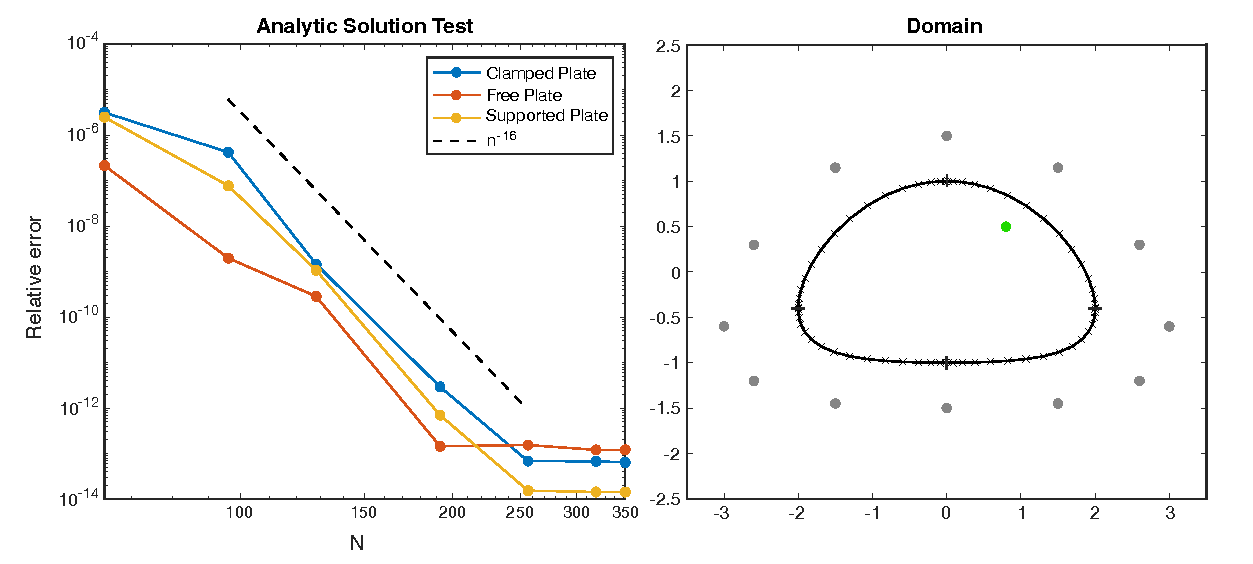
\includegraphics[scale=0.83]{convergence_figure.pdf}
\caption{Convergence of the three boundary integral equations ($k = 8, \nu = 1/3$) as a function of the number of discretization points. The solutions converge at sixteenth order using a combination of smooth and log quadratures. The solutions were solved on a domain shaped like a droplet (right), with the green dot representing the location of the point source and the grey dots representing the locations where the error was measured. The discretization on the right uses four 16-point Gauss-Legendre panels, which was the coarsest discretization that was tested. }\label{convergence_figure}
\end{figure}

\begin{figure}[ht]
\hspace{-1cm}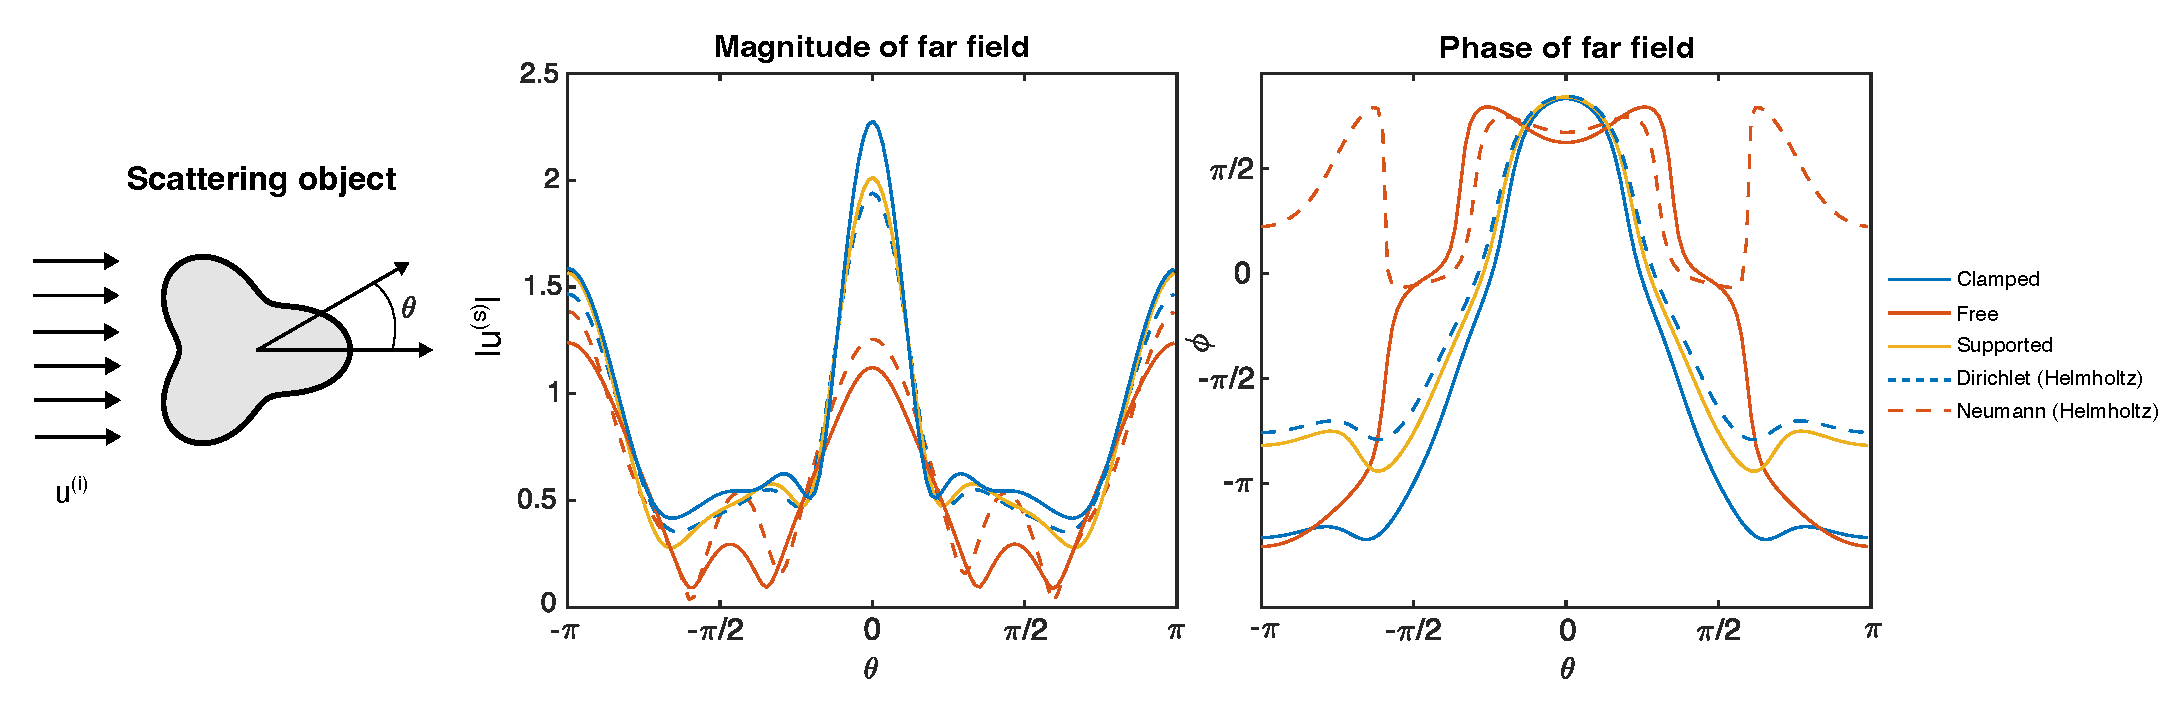
\includegraphics[scale=0.5]{far_field_starfish3arm_1_edited.pdf}
\caption{Comparison of boundary conditions on a starfish for wavenumber $k = 3$. Different boundary conditions lead to different far field patterns. The clamped plate creates the darkest shadow and the strongest backscatter. Meanwhile, in the free plate, the shadow and the backscatter are roughly equal in magnitude. The far field pattern generated by the supported plate is notably similar to that generated by the Helmholtz equation with Dirichlet boundary conditions.   }\label{farfield1}
\end{figure}


To investigate the qualitative differences in different boundary conditions, we plot the far-field patterns that are generated when a wave is scattered by an object, in this case, a tripedal starfish (Figure \ref{farfield1}). The parametrization for a generic starfish is given by
\begin{align}
    x(t) &= x_0 + (1+ A \cos(n t)) \cos(t) \\
    y(t) &= y_0 + (1+ A \cos(n t)) \sin(t)
\end{align}
where $t \in [0, 2\pi)$, the size of the arms is given by $A$, the center of the starfish is given by $(x_0, y_0)$, and the number of appendages is given by $n$ (in this case $n= 3$). We let the incoming field be $u^{(i)}(\mathbf{x}) := e^{i \mathbf{k} \cdot \mathbf{x}}$ where $\mathbf{k} = (3, 0)$ and set the boundary conditions for the scattered field, $u^{(s)}$ to be the negative of the boundary data corresponding to the plane wave, so that the boundary data of the total field, $u=u^{(i)}+u^{(s)}$, is equal to zero. Because the Yukawa part of the Green's function \eqref{greens} decays exponentially away from the boundary, the solutions far away from the boundary will naturally look like solutions to the Helmholtz equation. The limiting behavior of the two-dimensional Helmholtz Green's function is $H_0^{(1)}(k|\mathbf{x}|) \sim \sqrt{\frac{2}{\pi k |\mathbf{x} | }} e^{i ( k |\mathbf{x} | - \frac{1}{4} \pi )} $ \cite{NIST}, therefore the far-field pattern of the Helmholtz scattering problem can be written as $u^{(s)} \sim  f(\theta) \frac{1}{ | \mathbf{x} | } e^{ i k | \mathbf{x} | } $. Taking $|\mathbf{x}|$ sufficiently large to guarantee we are in the Helmholtz regime and multiplying the scattered field by $|\mathbf{x} | e^{- i k | \mathbf{x} |}$, we can easily recover the far-field pattern $f(\theta)$. To understand how the solutions to flexural wave BVPs differ from Helmholtz, we also plot the far field patterns for the Helmholtz scattering problem with Dirichlet and Neumann boundary conditions. Lastly, the phase of the outgoing solutions is calculated using the formula $\phi = \arctan \left( \Im(u^{(s)}) / \Re(u^{(s)}) \right)$.






The selection of boundary conditions leads to qualitatively different patterns in the far-field (Figures \ref{farfield1} and \ref{farfield2}). The clamped plate has a disruptive effect on the incoming wave, leading to the darkest shadow and the strongest backscatter. This effect is even stronger than the analogous Dirichlet problem for the Helmholtz equation. Meanwhile, the free plate had the lightest shadow and weakest backscatter, suggesting that the wave is able to ``pass'' through the object with less disturbance. Again, this passivity is stronger in the flexural wave case than in the analogous Neumann problem for the Helmholtz equation. The far field of the supported plate is surprisingly similar to that of the Dirichlet problem for the Helmholtz equation. 

The phase of the far field varies to an even greater extent than the magnitude. In some parts of the far-field ($\theta = \pm \pi/2$), the clamped and free plate are roughly half a period out of phase, while in other parts of the far-field ($\theta = \pi$), the clamped and far fields are in phase. This is a large contrast from the Helmholtz case, where the Dirichlet and Neumann problems are once again half a period out of phase at the angle $\theta = \pi$. 

\begin{figure}[ht]
\hspace{-1cm}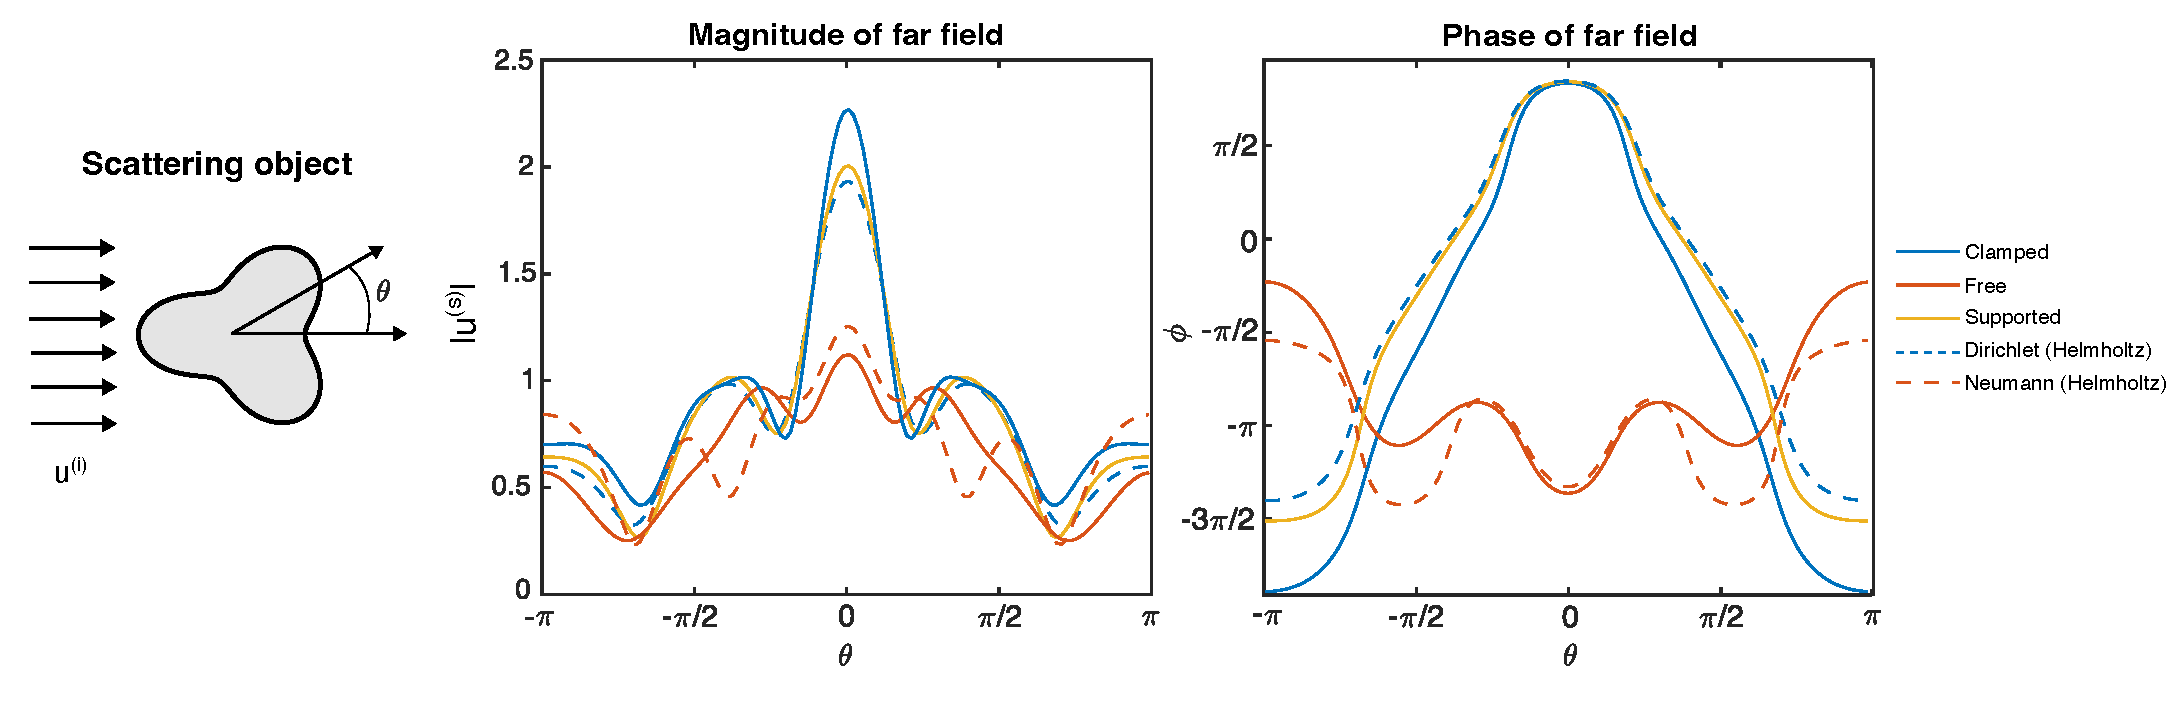
\includegraphics[scale=0.5]{far_field_starfish3arm_2_edited.pdf}
\caption{Far field patterns generated by the same wavenumber and starfish rotated by $\pi/3$. Again, the wavenumber is $k = 3$. In this case, the backscatter is not quite as strong due to the change in the orientation in the starfish. Instead, there is one main peak corresponding to the shadow and two smaller peaks corresponding to waves which are deflected off of the arms of the starfish. Again, the far field pattern of the supported plate is similar to the far field pattern of the Helmholtz equation with Dirichlet boundary conditions. }\label{farfield2}
\end{figure}

A convenient feature of the boundary integral equations described in this paper is that, after suitable discretization, they are amenable to standard techniques from fast algorithms such as {\it inter alia} fast multipole methods \cite{fmm,fmm1,fmm2,fmm3,fmm4,fmm6,fmm7,fmm8}, and fast direct solvers~\cite{darve2013jsc,aminfar2016fast,hackbusch2000,hackbusch2002,hackbusch2002anm,darve2013jsc,gu2001,sheng2007,gu2007,xia2009,dewilde2010,martinsson2019fast,fds1,fds2,fds3,fds4,fds5,fds6,fds7,fds8,marple2016fast,rss,bremer2015high,gopal2022accelerated}. As a demonstration of this, we conclude our numerical illustrations with an example of the BIE applied to a large scale problem. In particular, we consider a plane wave scattering off of 101 inclusions with free plate boundary  
conditions. The resulting discretized system has 76,480 unknowns. To accelerate the computation and reduce the overall memory cost we use a simplified (and slightly modified) version of skeletonization with proxy surfaces, see for example \cite{martinsson2019fast}. The results are shown in Figure \ref{multiplescattering}. We remark that a `branching' structure is visible in the magnitude of the field. For simpler models this structure has been previously observed both experimentally and numerically in the context of flexural waves \cite{Jose2022, Jose2023, matula1995energy, Darabi2018}. Our formulation allows for further exploration of this phenomenon.

\begin{figure}[ht]
\centering
\includegraphics[scale=1.2]{multiple_scattering_final_3.pdf}
\caption{ Flexural wave scattering by a collection of 101 starfish-shaped cavities in a thin elastic plate. Free plate BCs are prescribed on the boundary of each starfish, allowing the wave to pass quite far into the array before being attenuated. The wavenumber of the incident wave is $k = 6$ and the angle of the incident wave ($\theta = \pi/4$) is depicted by the black arrow.    }\label{multiplescattering}
\end{figure}





\clearpage
\section{Discussion} \label{discussion}

In this paper, we have presented integral equation methods for solving flexural wave problems for three common sets of boundary
conditions, either by extending existing methods as in the case of the clamped and supported plates, or by developing new methods in the case of the free plate. For the latter, we have used an integral representation that incorporates the composition of a standard layer potential with the Hilbert transform in order to obtain a second kind integral equation. Since the Hilbert transform offers another set of options for kernels in the integral representation, we believe this method may be useful more generally for the development of new integral representations for BVPs. Though not the focus of this study, interior problems can also be accurately solved using these methods. Given a compact geometry, one can
find its interior resonant modes by computing the roots of the Fredholm determinant~\cite{zhao2015robust,Askham2020}.
Further, the representations should be applicable to the static ($k=0$) case, a classical model
in elasticity.

Our hope is that these methods will be useful to researchers interested in flexural waves
in both the applied engineering and glaciological communities. The methods are high-order accurate and 
can be readily extended to larger systems using existing fast algorithms. The evolution of 
sea ice and ice shelves is a multiscale phenomenon, and there is a growing desire to model 
coupled problems at multiple scales \cite{Banwell2023}. In order to understand how smaller processes involving ice-shelf flexure may have an effect on the the large-scale climate, it is necessary to be able to solve large problems quickly. Fast algorithms based on second-kind integral equation representations are well-equipped to handle these large scattering problems, and we expect these methods to be effective in modeling wave propagation in sea ice and ice shelves. We anticipate that this paper will be the first in a series that leverages integral equations to solve wave scattering problems related to the modeling of sea ice. 



The boundary integral equations derived above were shown to be second kind for sufficiently smooth
geometries, requiring up to four absolutely continuous derivatives in the boundary parameterization
for the Taylor series estimates. There are a number of 
further questions to explore, including the behavior of the representations on geometries of lower
regularity; the solvability of the boundary integral equations and whether or not they are subject
to spurious resonances or spurious near-resonances~\cite{zhao2015robust}; and the uniqueness properties 
of solutions to the exterior free plate problem. The authors plan to explore the development of
representations for these problems with weaker dependence on the smoothness of the curve. Such representations may be necessary for the treatment
of domains with geometric singularities, like corners and cracks. The solvability of the integral equations will
be treated in future work, including the characterization of any nullspaces and resonances of the equations
for both the $k\ne 0$ and $k=0$ cases. The application of these methods to transmitting flexural
waves is also being vigorously pursued. 


\section{Code availability}

The integral equations were implemented and solved in \texttt{ChunkIE}, a MATLAB integral equations toolbox (\url{https://github.com/fastalgorithms/chunkie}). The examples from this paper may be found at \url{https://github.com/askhamwhat/flex-paper-examples}. 

\section{Acknowledgements}

We would like to thank Douglas MacAyeal, Shidong Jiang, Tristan Goodwill, and Mary Silber for many useful discussions. P.N. would like to acknowledge the support of the National Science Foundation (NSF) under Grant No. 2332479. J.G. Hoskins would like to thank the American Institute of Mathematics and, in particular, John Fry for hosting him on Bock Cay during the SQuaREs program, where parts of this work were completed. 
\appendix

\section{Heuristic strategy for deriving the integral kernels}

    Here we review the strategy  mentioned in~\cite{farkas}  for deriving suitable integral kernels $K_i$ and
    describe its extension to the free and supported plate problems. In order to derive the kernels, it is useful to look at the Green's function on a domain with infinitely many degrees of symmetry. Consider the upper half-plane $\Omega := \{ (x_1,x_2) | x_2 \geq 0 \}$. In this geometry, the convolutions
    that define layer potentials can be understood in terms of the Fourier transforms of the 
    integral kernels in the $x_1$ direction; for an application, see~\cite{oneil2014efficient}. 
    The Green's function has the Sommerfeld integral identity~\cite{sommerfeld1949partial}:  
    \begin{align}   G(\mathbf{x},\mathbf{y}) &= \int^{\infty}_{-\infty      }  \hat{G}(\xi,x_2) \exp{(i\xi (x_1 - y_1 ))} \, \dd \xi \label{sommerfeld} 
\end{align}
where
\begin{align}
    \hat{G}(\xi,x_2) &= \frac{1}{8 \pi k^2}  \left ( \frac{\exp{(- x_2 \sqrt{\xi^2 - k^2}) }}{\sqrt{\xi^2 - k^2}} - \frac{\exp{(-x_2 \sqrt{\xi^2 + k^2 }) }}{\sqrt{\xi^2 + k^2}} \right )
\end{align}
given $\mathbf{x} = (x_1,x_2)$ and $\mathbf{y}=(y_1,0)$. Because the expression for $\hat{G}$ is separated in the $x_1$ and $x_2$ directions,
it is simple to compute a similar Fourier transform of normal and tangential derivatives of the Green's function.

For any candidate kernel, $K_i$, given as some linear combination of derivatives of the Green's function, it is then possible 
to evaluate the $x_2\to 0^+$ limit of the boundary conditions applied to that kernel in terms of its 
Fourier transform.
Generally, the asymptotic expansion of this limit will include terms of the form $\xi^m$ or $\xi^m \sign(\xi)$ for $m \in \mathbb{Z}$ as 
$\xi \rightarrow \pm \infty$ which can be used to characterize the corresponding boundary integral operator: 
positive values of $m$ correspond to hyper-singular boundary integral kernels in the $\mathbf{K}$ matrix or differential operators
in the $\mathbf{D}$ matrix and a non-zero constant term in the expansion corresponds to a constant 
jump while a signed constant corresponds to a Hilbert transform. The goal in integral kernel design is that this limiting
system should be second kind. Ideally, $D_{ii}+K_{ii}$ should have a constant
term and no higher order terms in the asymptotic expansion while $D_{ij}+K_{ij}$
for $i\ne j$ should have only $o(1)$ terms. 

For example, the $\xi \to \pm \infty$ asymptotic expansions of some derivatives of
$G$ are below 
\begin{align}
    \lim_{x_2\to 0^+} \widehat{G_{n_\by n_\by n_\by}} &= \frac{1}{2} + o(1)\\
    \lim_{x_2\to 0^+} \widehat{G_{n_\by \tau_\by \tau_\by}} &= 0 + o(1)\\
    \lim_{x_2\to 0^+} \widehat{G_{n_\bx n_\by n_\by n_\by}} &= \frac{3}{4} |\xi| + o(1) \\
    \lim_{x_2\to 0^+} \widehat{G_{n_\bx n_\by \tau_\by \tau_\by}} &= -\frac{1}{4} |\xi| + o(1) \; .     
\end{align}
From these, we see that the $K_1$ kernel for the clamped plate problem, 
$K_1 = G_{n_\by n_\by n_\by} + 3 G_{n_\by \tau_\by \tau_\by}$, should have 
\begin{align}
    \widehat{D_{11} + K_{11}} &= \frac{1}{2} + o(1) \\
    \widehat{D_{21} + K_{21}} &= o(1) \; ,
\end{align}
as desired. 

Here we make a few observations. The first is that this analysis predicts,
correctly, that $D_{11} + \mathcal{K}_{11}$ should be second kind, with the constant in the
Fourier transform corresponding to the interior jump for this geometry. The second
is that the curvature-dependent term in $D_{21} + \mathcal{K}_{21}$ is not predicted because the
boundary is flat. Finally, we note that it is a general fact that the asymptotic
expansions contain terms of the form $\xi^m$ if the number of normal derivatives is
odd and of the form $\xi^m\sign (\xi)$ if the number is even. That is why the linear
combination of a term with three normal derivatives and a term with one normal
derivative is able to achieve cancellations in the singular parts. 

The effect of curvature can be better understood by considering the analogous
problem on the disk, where the Fourier series of the Green's function can be written using Graf's addition formula: 
\begin{align}
    G(\mathbf{x}, \mathbf{y}) = \frac{1}{2k^2} \sum_{n=-\infty}^\infty \left[ \frac{i}{4} H_n^{(1)}(kr_\mathbf{x})J_n(kr_\mathbf{y}) - \frac{1}{2\pi} K_n(kr_\mathbf{x}) I_n(kr_\mathbf{y}) \right] \exp{(in\alpha)} \label{grafs} 
\end{align}
subject to $r_\mathbf{x} > r_\mathbf{y}$, where $r_\mathbf{x}$ is the target radius, $r_\mathbf{y}$ is the source radius, and $\alpha$ is the angle between the source and the target. As above, the separated representation allows for relatively
straightforward calculations of normal and tangential derivatives. The asymptotic expansions 
(as $n \to \pm \infty$) of the Fourier coefficients can then be computed and a similar analysis 
applied. If the disk radius, $r_\by$, appears in the asymptotics, this corresponds to a curvature
dependence. This can help guide the derivation of the jump conditions on general curves.

For the free plate problem, we use a slightly different representation of the form
$\mathcal{K}_1 = \mathcal{K}_1^a + \mathcal{K}_1^b \mathcal{H}$. Because the Fourier
symbol of the Hilbert transform is $-i\sign(\xi)$, such a representation allows us to
cancel the singular parts of $K_1^a$ and $K_1^b$, even though $K_1^a$ has one normal
derivative and $K_1^b$ has none. As observed in Section~\ref{freesection}, this
effect can be understood for general curves by applying the Poincar\'{e}-Bertrand formula
and adding and subtracting the Hilbert transform from appropriate parts of the kernel. 
This Hilbert transform-based strategy then gives new degrees of freedom
in the design of integral kernels on general curves and surfaces and is likely applicable to 
integral kernel design for a variety of problems. 


\section{Formulae for the derivatives of the biharmonic Green's function} 
Let us denote the biharmonic Green's function as $G^{B} = \frac{1}{16\pi} \pmb{r}^2 \ln(\pmb{r}^2) $, where $\pmb{r}^2 = \pmb{r}\cdot \pmb{r}$ and $\pmb{r} = \mathbf{x}-\mathbf{y}$ is the distance between the target and the source. For the sake of completeness, we provide formulae for the derivatives of the biharmonic Green's function, which are used to analyze the leading order behavior of the flexural wave kernels: 
\subsection{Clamped plate kernels} \label{appclamped}
First, we provide the following derivatives of $G^{B}$ used in the integral equation for the clamped plate (Theorem \ref{clampedsmooth}).
\begin{align}
    G^{B}_{n_\mathbf{y} n_\mathbf{y}} &= \frac{1}{4\pi} \frac{[\pmb{r}\cdot  n(\mathbf{y}) ]^2}{\pmb{r}^2} + \frac{1}{8\pi}\ln(\pmb{r}^2) + \frac{1}{8\pi} \\
    G^{B}_{\tau_\mathbf{y} \tau_\mathbf{y}} &= \frac{1}{4\pi} \frac{[\pmb{r}\cdot \tau(\mathbf{y})]^2}{\pmb{r}^2} + \frac{1}{8\pi}\ln(\pmb{r}^2) + \frac{1}{8\pi}\\
    G^{B}_{n_\mathbf{x} n_\mathbf{y} n_\mathbf{y}} &= \frac{1}{2\pi} \frac{[\pmb{r}\cdot n(\mathbf{y})][n(\mathbf{y}) \cdot  n(\mathbf{x}) ]}{\pmb{r}^2} - \frac{1}{2\pi} \frac{[\pmb{r}\cdot  n(\mathbf{x}) ][\pmb{r}\cdot n(\mathbf{y})]^2}{\pmb{r}^4} +\frac{1}{4\pi}\frac{\pmb{r}\cdot  n(\mathbf{x}) }{\pmb{r}^2}\\
    G^{B}_{n_\mathbf{x} \tau_\mathbf{y} \tau_\mathbf{y}} &= \frac{1}{2\pi} \frac{[\pmb{r}\cdot \tau(\mathbf{y})][\tau(\mathbf{y}) \cdot  n(\mathbf{x}) ]}{\pmb{r}^2} - \frac{1}{2\pi} \frac{[\pmb{r}\cdot  n(\mathbf{x}) ][\pmb{r}\cdot \tau(\mathbf{y})]^2}{\pmb{r}^4} +\frac{1}{4\pi}\frac{\pmb{r}\cdot  n(\mathbf{x}) }{\pmb{r}^2}\\
    G^{B}_{n_\mathbf{y} n_\mathbf{y} n_\mathbf{y}} &= -\frac{3}{4\pi} \frac{[\pmb{r}\cdot n(\mathbf{y})]}{\pmb{r}^2} + \frac{1}{2\pi} \frac{[\pmb{r}\cdot n(\mathbf{y})]^3}{\pmb{r}^4} \\
    G^{B}_{ n_\mathbf{y} \tau_\mathbf{y} \tau_\mathbf{y}} &=  \frac{1}{2\pi} \frac{[\pmb{r}\cdot  n(\mathbf{y}) ][\pmb{r}\cdot \tau(\mathbf{y})]^2}{\pmb{r}^4} -\frac{1}{4\pi}\frac{\pmb{r}\cdot  n(\mathbf{y}) }{\pmb{r}^2}\\
      G^{B}_{n_\mathbf{x} n_\mathbf{y} n_\mathbf{y} n_\mathbf{y}} &= -\frac{3}{4\pi} \frac{ n(\mathbf{x}) \cdot  n(\mathbf{y}) }{\pmb{r}^2} + \frac{3}{2\pi} \frac{[\pmb{r}\cdot  n(\mathbf{y}) ][\pmb{r}\cdot  n(\mathbf{x}) ]}{\pmb{r}^4}+ \frac{3}{2\pi} \frac{[\pmb{r}\cdot  n(\mathbf{y}) ]^2 [ n(\mathbf{x})  \cdot  n(\mathbf{y}) ]}{\pmb{r}^4} \nonumber \\
      &\qquad -\frac{2}{\pi} \frac{[\pmb{r} \cdot n(\mathbf{y})]^3[\pmb{r}\cdot n(\mathbf{x})]}{\pmb{r}^6} \\
    G^B_{n_\mathbf{x} n_\mathbf{y} \tau_\mathbf{y} \tau_\mathbf{y}} &=  \frac{1}{2\pi} \frac{[n(\mathbf{x}) \cdot n(\mathbf{y})][\pmb{r}\cdot \tau(\mathbf{y})]^2}{\pmb{r}^4} + \frac{1}{\pi} \frac{[\pmb{r}\cdot n(\mathbf{y})][\pmb{r}\cdot \tau(\mathbf{y})][n(\mathbf{x}) \cdot \tau(\mathbf{y})]}{\pmb{r}^4} \nonumber \\
    &\qquad - \frac{2}{\pi} \frac{[\pmb{r}\cdot n(\mathbf{y})][\pmb{r}\cdot \tau(\mathbf{y})]^2 [\pmb{r}\cdot n(\mathbf{x})]}{\pmb{r}^6} - \frac{1}{4\pi} \frac{n(\mathbf{x}) \cdot n(\mathbf{y}) }{\pmb{r}^2} \nonumber \\
    &\qquad + \frac{1}{2\pi} \frac{[\pmb{r}\cdot n(\mathbf{y})][\pmb{r}\cdot n(\mathbf{x})]}{\pmb{r}^4} 
\end{align}

\subsection{Free plate kernels} \label{appfree}
First, we provide the following derivatives of $G^{B}$ used in the integral equation for the clamped plate (Theorem \ref{freesmooth}).
\begin{align}
    G^{B}_{n_\mathbf{x} n_\mathbf{x}} &= \frac{1}{4\pi} \frac{[\pmb{r}\cdot  n(\mathbf{x}) ]^2}{\pmb{r}^2} + \frac{1}{8\pi}\ln(\pmb{r}^2) + \frac{1}{8\pi} \\
    G^{B}_{\tau_\mathbf{x} \tau_\mathbf{x}} &= \frac{1}{4\pi} \frac{[\pmb{r}\cdot \tau(\mathbf{x})]^2}{\pmb{r}^2} + \frac{1}{8\pi}\ln(\pmb{r}^2) + \frac{1}{8\pi}\\
    G^{B}_{n_\mathbf{x} n_\mathbf{x} n_\mathbf{y}} &= -\frac{1}{2\pi} \frac{[\pmb{r}\cdot n(\mathbf{x})][n(\mathbf{x}) \cdot  n(\mathbf{y}) ]}{\pmb{r}^2} + \frac{1}{2\pi} \frac{[\pmb{r}\cdot  n(\mathbf{y}) ][\pmb{r}\cdot n(\mathbf{x})]^2}{\pmb{r}^4} -\frac{1}{4\pi}\frac{\pmb{r}\cdot  n(\mathbf{y}) }{\pmb{r}^2}\\
    G^{B}_{\tau_\mathbf{x} \tau_\mathbf{x} n_\mathbf{y}} &= -\frac{1}{2\pi} \frac{[\pmb{r}\cdot \tau(\mathbf{x})][\tau(\mathbf{x}) \cdot  n(\mathbf{y}) ]}{\pmb{r}^2} + \frac{1}{2\pi} \frac{[\pmb{r}\cdot  n(\mathbf{y}) ][\pmb{r}\cdot \tau(\mathbf{x})]^2}{\pmb{r}^4} -\frac{1}{4\pi}\frac{\pmb{r}\cdot  n(\mathbf{y}) }{\pmb{r}^2}\\
    G^{B}_{n_\mathbf{x} n_\mathbf{x} \tau_\mathbf{y}} &= -\frac{1}{2\pi} \frac{[\pmb{r}\cdot  n(\mathbf{x}) ][ n(\mathbf{x})  \cdot  \tau(\mathbf{y}) ]}{\pmb{r}^2} + \frac{1}{2\pi} \frac{[\pmb{r}\cdot  \tau(\mathbf{y}) ][\pmb{r}\cdot  n(\mathbf{x}) ]^2}{\pmb{r}^4} -\frac{1}{4\pi}\frac{\pmb{r}\cdot  \tau(\mathbf{y}) }{\pmb{r}^2}\\
     G^{B}_{\tau_\mathbf{x} \tau_\mathbf{x} \tau_\mathbf{y}} &= -\frac{1}{2\pi} \frac{[\pmb{r}\cdot \tau(\mathbf{x})][\tau(\mathbf{x}) \cdot  \tau(\mathbf{y}) ]}{\pmb{r}^2} + \frac{1}{2\pi} \frac{[\pmb{r}\cdot  \tau(\mathbf{y}) ][\pmb{r}\cdot \tau(\mathbf{x})]^2}{\pmb{r}^4} -\frac{1}{4\pi}\frac{\pmb{r}\cdot  \tau(\mathbf{y}) }{\pmb{r}^2}\\
    G^{B}_{n_\mathbf{x} n_\mathbf{x} n_\mathbf{x}} &= \frac{3}{4\pi} \frac{\pmb{r}\cdot n(\mathbf{x})}{\pmb{r}^2} - \frac{1}{2\pi} \frac{[\pmb{r}\cdot n(\mathbf{x})]^3}{\pmb{r}^4} \\
    G^{B}_{n_\mathbf{x} \tau_\mathbf{x} \tau_\mathbf{x} } &=  - \frac{1}{2\pi} \frac{[\pmb{r}\cdot  n(\mathbf{x}) ][\pmb{r}\cdot \tau(\mathbf{x})]^2}{\pmb{r}^4} +\frac{1}{4\pi}\frac{\pmb{r}\cdot  n(\mathbf{x}) }{\pmb{r}^2}\\
    G^{B}_{n_\mathbf{x} n_\mathbf{x} n_\mathbf{x} n_\mathbf{y}} &= -\frac{3}{4\pi} \frac{ n(\mathbf{x}) \cdot  n(\mathbf{y}) }{\pmb{r}^2} + \frac{3}{2\pi} \frac{[\pmb{r}\cdot  n(\mathbf{y}) ][\pmb{r}\cdot  n(\mathbf{x}) ]}{\pmb{r}^4}+ \frac{3}{2\pi} \frac{[\pmb{r}\cdot  n(\mathbf{x}) ]^2 [ n(\mathbf{x})  \cdot  n(\mathbf{y}) ]}{\pmb{r}^4} \nonumber \\
    &\qquad -\frac{2}{\pi} \frac{[\pmb{r} \cdot n(\mathbf{x})]^3[\pmb{r}\cdot n(\mathbf{y})]}{\pmb{r}^6} \\
    G^{B}_{n_\mathbf{x} \tau_\mathbf{x} \tau_\mathbf{x}  n_\mathbf{y}} &= \frac{1}{2\pi} \frac{[\pmb{r} \cdot \tau(\mathbf{x})]^2 [ n(\mathbf{x})  \cdot  n(\mathbf{y}) ]}{\pmb{r}^4} + \frac{1}{\pi} \frac{[\pmb{r}\cdot \tau(\mathbf{x}) ][\tau(\mathbf{x})\cdot  n(\mathbf{y}) ] [\pmb{r} \cdot  n(\mathbf{x}) ] }{\pmb{r}^4} \nonumber \\
    &\qquad - \frac{2}{\pi} \frac{[\pmb{r} \cdot  n(\mathbf{y}) ][\pmb{r} \cdot  n(\mathbf{x}) ] [\pmb{r} \cdot \tau(\mathbf{x})]^2 }{\pmb{r}^6} -\frac{1}{4\pi} \frac{ n(\mathbf{x})  \cdot  n(\mathbf{y}) }{\pmb{r}^2 }+ \frac{1}{2\pi} \frac{[\pmb{r} \cdot  n(\mathbf{y}) ][\pmb{r} \cdot  n(\mathbf{x}) ]}{\pmb{r}^4}\\
     G^{B}_{n_\mathbf{x} n_\mathbf{x} n_\mathbf{x} \tau_\mathbf{y}} &= -\frac{3}{4\pi}\frac{ n(\mathbf{x})  \cdot  \tau(\mathbf{y}) }{\pmb{r}^2} + \frac{3}{2\pi} \frac{[\pmb{r}\cdot  n(\mathbf{x}) ][\pmb{r}\cdot  \tau(\mathbf{y}) ]}{\pmb{r}^4} + \frac{3}{2\pi} \frac{[\pmb{r}\cdot  n(\mathbf{x}) ]^2(  n(\mathbf{x})  \cdot  \tau(\mathbf{y}) )}{\pmb{r}^4} \nonumber \\
    &\qquad -\frac{2}{\pi}\frac{[\pmb{r}\cdot  \tau(\mathbf{y})  ][\pmb{r} \cdot  n(\mathbf{x}) ]^3}{\pmb{r}^6}\\
     G^{B}_{n_\mathbf{x} \tau_\mathbf{x} \tau_\mathbf{x} \tau_\mathbf{y} } &= \frac{1}{\pi} \frac{[\pmb{r}\cdot  n(\mathbf{x})  ][\pmb{r}\cdot \tau(\mathbf{x})] [\tau(\mathbf{x})\cdot  \tau(\mathbf{y}) ]}{\pmb{r}^4}+ \frac{1}{2\pi }\frac{( \tau(\mathbf{y})  \cdot  n(\mathbf{x}) ) [\pmb{r} \cdot \tau(\mathbf{x})]^2}{\pmb{r}^4} \nonumber \\
    &\qquad - \frac{2}{\pi} \frac{[\pmb{r}\cdot  n(\mathbf{x}) ][\pmb{r} \cdot  \tau(\mathbf{y}) ][\pmb{r} \cdot \tau(\mathbf{x})]^2}{\pmb{r}^6} - \frac{1}{4\pi} \frac{ \tau(\mathbf{y})  \cdot  n(\mathbf{x}) }{\pmb{r}^2} + \frac{1}{2\pi} \frac{[\pmb{r} \cdot  n(\mathbf{x}) ] [\pmb{r} \cdot  \tau(\mathbf{y})  ]}{\pmb{r}^4} 
\end{align}

\subsection{Supported plate kernels} \label{appsupported}
First, we provide the following derivatives of $G^{B}$ used in the integral equation for the supported plate (Theorem \ref{supportedsmooth}).
\begin{align}
        G^{B}_{n_\mathbf{y} } &= - \frac{1}{8\pi} [\pmb{r} \cdot n(\mathbf{y})] \ln(\pmb{r}^2) -  \frac{1}{8\pi} [\pmb{r} \cdot n(\mathbf{y})]    \\
        G^{B}_{\tau_\mathbf{y} } &= - \frac{1}{8\pi} [\pmb{r} \cdot \tau(\mathbf{y})] \ln(\pmb{r}^2) -  \frac{1}{8\pi} [\pmb{r} \cdot \tau(\mathbf{y})]    \\
        G^{B}_{n_\mathbf{y} n_\mathbf{y}} &= \frac{1}{4\pi} \frac{[\pmb{r}\cdot  n(\mathbf{y}) ]^2}{\pmb{r}^2} + \frac{1}{8\pi}\ln(\pmb{r}^2) + \frac{1}{8\pi} \\
    G^{B}_{n_\mathbf{y} n_\mathbf{y} n_\mathbf{y}} &= -\frac{3}{4\pi} \frac{[\pmb{r}\cdot n(\mathbf{y})]}{\pmb{r}^2} + \frac{1}{2\pi} \frac{[\pmb{r}\cdot n(\mathbf{y})]^3}{\pmb{r}^4} \\
    G^{B}_{ n_\mathbf{y} \tau_\mathbf{y} \tau_\mathbf{y}} &=  \frac{1}{2\pi} \frac{[\pmb{r}\cdot  n(\mathbf{y}) ][\pmb{r}\cdot \tau(\mathbf{y})]^2}{\pmb{r}^4} -\frac{1}{4\pi}\frac{\pmb{r}\cdot  n(\mathbf{y}) }{\pmb{r}^2} \\
  G^{B}_{n_\mathbf{x} n_\mathbf{x} n_\mathbf{y}} &= -\frac{1}{2\pi} \frac{[\pmb{r}\cdot n(\mathbf{x})][n(\mathbf{x}) \cdot  n(\mathbf{y}) ]}{\pmb{r}^2} + \frac{1}{2\pi} \frac{[\pmb{r}\cdot  n(\mathbf{y}) ][\pmb{r}\cdot n(\mathbf{x})]^2}{\pmb{r}^4} -\frac{1}{4\pi}\frac{\pmb{r}\cdot  n(\mathbf{y}) }{\pmb{r}^2}\\
    G^{B}_{\tau_\mathbf{x} \tau_\mathbf{x} n_\mathbf{y}} &= -\frac{1}{2\pi} \frac{[\pmb{r}\cdot \tau(\mathbf{x})][\tau(\mathbf{x}) \cdot  n(\mathbf{y}) ]}{\pmb{r}^2} + \frac{1}{2\pi} \frac{[\pmb{r}\cdot  n(\mathbf{y}) ][\pmb{r}\cdot \tau(\mathbf{x})]^2}{\pmb{r}^4} -\frac{1}{4\pi}\frac{\pmb{r}\cdot  n(\mathbf{y}) }{\pmb{r}^2}\\
    G^{B}_{n_\mathbf{x} n_\mathbf{x} \tau_\mathbf{y}} &= -\frac{1}{2\pi} \frac{[\pmb{r}\cdot  n(\mathbf{x}) ][ n(\mathbf{x})  \cdot  \tau(\mathbf{y}) ]}{\pmb{r}^2} + \frac{1}{2\pi} \frac{[\pmb{r}\cdot  \tau(\mathbf{y}) ][\pmb{r}\cdot  n(\mathbf{x}) ]^2}{\pmb{r}^4} -\frac{1}{4\pi}\frac{\pmb{r}\cdot  \tau(\mathbf{y}) }{\pmb{r}^2}\\
     G^{B}_{\tau_\mathbf{x} \tau_\mathbf{x} \tau_\mathbf{y}} &= -\frac{1}{2\pi} \frac{[\pmb{r}\cdot \tau(\mathbf{x})][\tau(\mathbf{x}) \cdot  \tau(\mathbf{y}) ]}{\pmb{r}^2} + \frac{1}{2\pi} \frac{[\pmb{r}\cdot  \tau(\mathbf{y}) ][\pmb{r}\cdot \tau(\mathbf{x})]^2}{\pmb{r}^4} -\frac{1}{4\pi}\frac{\pmb{r}\cdot  \tau(\mathbf{y}) }{\pmb{r}^2}\\
    G^{B}_{n_\mathbf{x} n_\mathbf{x} n_\mathbf{y} n_\mathbf{y}} &= \frac{1}{2\pi} \frac{[n(\mathbf{x})\cdot n(\mathbf{y})]^2}{\pmb{r}^2} - \frac{2}{\pi} \frac{[\pmb{r}\cdot n(\mathbf{x})][\pmb{r} \cdot n(\mathbf{y})][n(\mathbf{x})\cdot n(\mathbf{y})]}{\pmb{r}^4} + \frac{1}{4\pi} \frac{1}{\pmb{r}^2} \nonumber \\
    &\qquad -\frac{1}{2\pi}\frac{[\pmb{r}\cdot n(\mathbf{y})]^2}{\pmb{r}^4} + \frac{2}{\pi} \frac{[\pmb{r}\cdot n(\mathbf{x})]^2[\pmb{r}\cdot n(\mathbf{y})]^2}{\pmb{r}^6} - \frac{1}{2\pi} \frac{[\pmb{r}\cdot n(\mathbf{x})]^2}{\pmb{r}^4}  \\
    G^{B}_{\tau_\mathbf{x} \tau_\mathbf{x} n_\mathbf{y} n_\mathbf{y}} &= \frac{1}{2\pi} \frac{[\tau(\mathbf{x})\cdot n(\mathbf{y})]^2}{\pmb{r}^2} - \frac{2}{\pi} \frac{[\pmb{r}\cdot \tau(\mathbf{x})][\pmb{r} \cdot n(\mathbf{y})][\tau(\mathbf{x})\cdot n(\mathbf{y})]}{\pmb{r}^4} + \frac{1}{4\pi} \frac{1}{\pmb{r}^2} \nonumber \\
    &\qquad -\frac{1}{2\pi}\frac{[\pmb{r}\cdot n(\mathbf{y})]^2}{\pmb{r}^4} + \frac{2}{\pi} \frac{[\pmb{r}\cdot \tau(\mathbf{x})]^2[\pmb{r}\cdot n(\mathbf{y})]^2}{\pmb{r}^6} - \frac{1}{2\pi} \frac{[\pmb{r}\cdot \tau(\mathbf{x})]^2}{\pmb{r}^4}  \\
  G^B_{n_{\mathbf{x}} n_{\mathbf{x}} n_{\mathbf{y}} n_{\mathbf{y}} n_{\mathbf{y}}} &= \frac{3}{2 \pi} \frac{\pmb{r} \cdot n(\mathbf{y})}{\pmb{r}^4} - \frac{6}{\pi} \frac{[\pmb{r} \cdot n(\mathbf{y})][\pmb{r}\cdot n(\mathbf{x})]^2}{\pmb{r}^6} + \frac{3}{\pi} \frac{[\pmb{r} \cdot n(\mathbf{y})][n(\mathbf{x}) \cdot n(\mathbf{y})]^2}{\pmb{r}^4} \nonumber \\
    &\qquad - \frac{12}{\pi} \frac{[\pmb{r}\cdot n(\mathbf{y})]^2 [\pmb{r} \cdot n( \mathbf{x}) ][n(\mathbf{x}) \cdot n(\mathbf{y})]}{\pmb{r}^6} - \frac{2}{\pi} \frac{[\pmb{r} \cdot n(\mathbf{y})]^3}{\pmb{r}^6} \nonumber \\
    &\qquad + \frac{12}{\pi} \frac{[\pmb{r} \cdot n(\mathbf{y})]^3 [\pmb{r}\cdot n(\mathbf{x})]^2}{\pmb{r}^8} + \frac{3}{\pi} \frac{[\pmb{r}\cdot n(\mathbf{x})][n(\mathbf{x}) \cdot n(\mathbf{y})]}{\pmb{r}^4} \label{Gnxnxnynyny} \\
    G^B_{\tau_{\mathbf{x}} \tau_{\mathbf{x}} n_{\mathbf{y}} n_{\mathbf{y}} n_{\mathbf{y}}} &= \frac{3}{2 \pi} \frac{\pmb{r} \cdot n(\mathbf{y})}{\pmb{r}^4} - \frac{6}{\pi} \frac{[\pmb{r} \cdot n(\mathbf{y})][\pmb{r}\cdot \tau(\mathbf{x})]^2}{\pmb{r}^6} + \frac{3}{\pi} \frac{[\pmb{r} \cdot n(\mathbf{y})][\tau(\mathbf{x}) \cdot n(\mathbf{y})]^2}{\pmb{r}^4} \nonumber \\
    &\qquad - \frac{12}{\pi} \frac{[\pmb{r}\cdot n(\mathbf{y})]^2 [\pmb{r} \cdot \tau( \mathbf{x}) ][\tau(\mathbf{x}) \cdot n(\mathbf{y})]}{\pmb{r}^6} - \frac{2}{\pi} \frac{[\pmb{r} \cdot n(\mathbf{y})]^3}{\pmb{r}^6} \nonumber \\
    &\qquad + \frac{12}{\pi} \frac{[\pmb{r} \cdot n(\mathbf{y})]^3 [\pmb{r}\cdot \tau(\mathbf{x})]^2}{\pmb{r}^8}+ \frac{3}{\pi} \frac{[\pmb{r}\cdot \tau(\mathbf{x})][\tau(\mathbf{x}) \cdot n(\mathbf{y})]}{\pmb{r}^4} \\
    G^B_{n_\mathbf{x} n_\mathbf{x} n_\mathbf{y} \tau_\mathbf{y} \tau_\mathbf{y}} &= \frac{2}{\pi} \frac{[n(\mathbf{x}) \cdot n(\mathbf{y}) ] [n(\mathbf{x}) \cdot \tau(\mathbf{y}) ] [\pmb{r} \cdot \tau(\mathbf{y})]}{\pmb{r}^4} - \frac{4}{\pi} \frac{[n(\mathbf{x}) \cdot n(\mathbf{y})][\pmb{r}\cdot \tau(\mathbf{y})]^2 [\pmb{r}\cdot n(\mathbf{x})]}{\pmb{r}^6} \nonumber \\
    &\qquad + \frac{1}{\pi} \frac{[\pmb{r} \cdot n(\mathbf{y}) ] [n(\mathbf{x}) \cdot \tau(\mathbf{y})]^2}{\pmb{r}^4} - \frac{8}{\pi} \frac{[\pmb{r} \cdot n(\mathbf{y})] [\pmb{r} \cdot \tau(\mathbf{y})] [\pmb{r}\cdot n(\mathbf{x})] [n(\mathbf{x}) \cdot \tau(\mathbf{y})]}{\pmb{r}^6} \nonumber \\
    &\qquad -\frac{2 }{\pi} \frac{[\pmb{r} \cdot n(\mathbf{y})] [\pmb{r}\cdot \tau(\mathbf{y})]^2}{\pmb{r}^6} + \frac{12}{\pi} \frac{[\pmb{r} \cdot n(\mathbf{y})][\pmb{r}\cdot \tau(\mathbf{y})]^2 [\pmb{r}\cdot n(\mathbf{x})]^2}{\pmb{r}^8} \nonumber \\
    &\qquad +\frac{1}{\pi} \frac{[n(\mathbf{x}) \cdot n(\mathbf{y})] [\pmb{r}\cdot n(\mathbf{x})]}{\pmb{r}^4} + \frac{1}{2\pi} \frac{\pmb{r} \cdot n(\mathbf{y})}{\pmb{r}^4}  - \frac{2}{\pi} \frac{[\pmb{r}\cdot n(\mathbf{y})][\pmb{r}\cdot n(\mathbf{x})]^2}{\pmb{r}^6} \\
    G^B_{\tau_\mathbf{x} \tau_\mathbf{x} n_\mathbf{y} \tau_\mathbf{y} \tau_\mathbf{y}} &= \frac{2}{\pi} \frac{[\tau(\mathbf{x}) \cdot n(\mathbf{y}) ] [\tau(\mathbf{x}) \cdot \tau(\mathbf{y}) ] [\pmb{r} \cdot \tau(\mathbf{y})]}{\pmb{r}^4} - \frac{4}{\pi} \frac{[\tau(\mathbf{x}) \cdot n(\mathbf{y})][\pmb{r}\cdot \tau(\mathbf{y})]^2 [\pmb{r}\cdot \tau(\mathbf{x})]}{\pmb{r}^6} \nonumber \\
    &\qquad + \frac{1}{\pi} \frac{[\pmb{r} \cdot n(\mathbf{y}) ] [\tau(\mathbf{x}) \cdot \tau(\mathbf{y})]^2}{\pmb{r}^4} - \frac{8}{\pi} \frac{[\pmb{r} \cdot n(\mathbf{y})] [\pmb{r} \cdot \tau(\mathbf{y})] [\pmb{r}\cdot \tau(\mathbf{x})] [\tau(\mathbf{x}) \cdot \tau(\mathbf{y})]}{\pmb{r}^6} \nonumber \\
    &\qquad -\frac{2 }{\pi} \frac{[\pmb{r} \cdot n(\mathbf{y})] [\pmb{r}\cdot \tau(\mathbf{y})]^2}{\pmb{r}^6} + \frac{12}{\pi} \frac{[\pmb{r} \cdot n(\mathbf{y})][\pmb{r}\cdot \tau(\mathbf{y})]^2 [\pmb{r}\cdot \tau(\mathbf{x})]^2}{\pmb{r}^8} \nonumber \\
    &\qquad +\frac{1}{\pi} \frac{[\tau(\mathbf{x}) \cdot n(\mathbf{y})] [\pmb{r}\cdot \tau(\mathbf{x})]}{\pmb{r}^4} + \frac{1}{2\pi} \frac{\pmb{r} \cdot n(\mathbf{y})}{\pmb{r}^4}  - \frac{2}{\pi} \frac{[\pmb{r}\cdot n(\mathbf{y})][\pmb{r}\cdot \tau(\mathbf{x})]^2}{\pmb{r}^6} 
\end{align}



\section{Derivation of jump conditions of the layer potentials}

So that this paper is self-contained, we repeat the derivation of jump conditions here. Given the arc-length parametrization $\pmb{\gamma}(t)$, let $\tau(t) := \tau(\pmb{\gamma}(t)) $ and $n(t) := n(\pmb{\gamma}(t)) $ be the unit tangent and normal vectors at $\pmb{\gamma}(t)$. Suppose that the target point is in the exterior of the domain while the source point is on the boundary:
\begin{align}
    \mathbf{x} &:= \pmb{\gamma}(t) + h n(t) \\
    \mathbf{y} &:= \pmb{\gamma}(t+s) 
\end{align}
As before, we expand $\pmb{r} =(\mathbf{x} - \mathbf{y})$ as:
\begin{align}
    \pmb{r} &= h n(t) - s \tau(t) + \frac{s^2}{2} \kappa n(t)  + \frac{s^3}{6}(\kappa' n(t) + \kappa^2 \tau(t) ) - \frac{s^4}{24} ((-\kappa'' + \kappa^3)n(t) - 3\kappa\kappa'\tau(t)) + \mathcal{O}(s^5) \label{rseries}
\end{align}
Next, we substitute expressions \eqref{tauseries} and \eqref{nseries} into the derivatives of the biharmonic Green's function. We obtain the following off surface asymptotics:
\begin{align}
    G^B_{n_\mathbf{x} n_\mathbf{x} n_\mathbf{x}}(\mathbf{x},\mathbf{y}) &=  \frac{3}{4 \pi} \frac{h}{h^2 + s^2} - \frac{1}{2\pi} \frac{h^3}{(h^2 + s^2)^2} + O(s^2) 
\end{align}
Integrating this kernel against some density $\sigma(\mathbf{y}) := \sigma(\pmb{\gamma}(t+s))$ in some region $[-\delta, \delta]$ along the curve and taking the limit as the target approaches the boundary:
\begin{align}
    \lim_{h \xrightarrow{} 0}  & \int^{+\delta}_{-\delta}   G_{n_\mathbf{x} n_\mathbf{x} n_\mathbf{x}}(\mathbf{x}, \mathbf{y}(s)) \sigma(\mathbf{y}(s)) \, \dd s \\
    &= \lim_{h \xrightarrow{} 0}  \left[ \sigma(\mathbf{x}) \int^{+\delta}_{-\delta} \left(  \frac{3}{4 \pi} \frac{h}{h^2 + s^2} - \frac{1}{2\pi} \frac{h^3}{(h^2 + s^2)^2} \right) ds \right] \label{jumpintegral1} \\
    &\qquad \qquad \qquad +  \lim_{h \xrightarrow{} 0}  \int^{+\delta}_{-\delta} (\sigma(\mathbf{y}) - \sigma(\mathbf{x}))  \left(  \frac{3}{4 \pi} \frac{h}{h^2 + s^2} - \frac{1}{2\pi} \frac{h^3}{(h^2 + s^2)^2} \right)  ds \bigg) \label{jumpintegral2} 
\end{align}
We deal with the second integral first. Because $\sigma(\mathbf{x})$ is continuous, \eqref{jumpintegral2} can be bounded by:
\begin{align}
    &\int^{+\delta}_{-\delta} (\sigma(\mathbf{y}) - \sigma(\mathbf{x}))  \left(  - \frac{3}{4 \pi} \frac{h}{h^2 + s^2} + \frac{1}{2\pi} \frac{h^3}{(h^2 + s^2)^2} \right)  ds \nonumber \\
    &\qquad\qquad\qquad\qquad\qquad\qquad \leq 2 \delta C \int^{+\delta}_{-\delta}   \left(  - \frac{3}{4 \pi} \frac{h}{h^2 + s^2} + \frac{1}{2\pi} \frac{h^3}{(h^2 + s^2)^2} \right)  ds
\end{align}
which goes to zero as $\delta \xrightarrow[]{} 0$. Next, we integrate \eqref{jumpintegral1}:
\begin{align}
    \lim_{h \xrightarrow{} 0} \bigg( \sigma(\mathbf{x}) \left( \frac{\delta h}{2\pi(\delta^2 + h^2)}  + \frac{1}{\pi} \arctan \frac{\delta}{h} \right) \bigg) ds = \frac{1}{2} \sigma(\mathbf{x})
\end{align}
Finally, we have the jump condition:
\begin{align}
    \lim_{\mathbf{x} \rightarrow \partial \Omega} \int_{\partial\Omega} G_{n_\mathbf{x}n_\mathbf{x}n_\mathbf{x}}(\mathbf{x},\mathbf{y}) \sigma(\mathbf{y}) \, \dd S(\mathbf{y}) = \frac{1}{2}\sigma(\mathbf{x}) + \int_{\partial\Omega} G_{n_\mathbf{x}n_\mathbf{x}n_\mathbf{x}}(\mathbf{x},\mathbf{y}) \sigma(\mathbf{y}) \, \dd S(\mathbf{y}) \label{jumpcond1}
\end{align}
Similar reasoning can be applied to obtain other jump conditions:
\begin{align}
    \lim_{\mathbf{x} \rightarrow \partial \Omega} \int_{\partial\Omega} G_{n_\mathbf{x}n_\mathbf{x}n_\mathbf{y}}(\mathbf{x},\mathbf{y}) \sigma(\mathbf{y}) \, \dd S(\mathbf{y}) &= -\frac{1}{2}\sigma(\mathbf{x}) + \int_{\partial\Omega} G_{n_\mathbf{x}n_\mathbf{x}n_\mathbf{y}}(\mathbf{x},\mathbf{y}) \sigma(\mathbf{y}) \, \dd S(\mathbf{y}) \\
    \lim_{\mathbf{x} \rightarrow \partial \Omega} \int_{\partial\Omega} G_{n_\mathbf{x}n_\mathbf{y}n_\mathbf{y}}(\mathbf{x},\mathbf{y}) \sigma(\mathbf{y}) \, \dd S(\mathbf{y}) &= \frac{1}{2}\sigma(\mathbf{x}) + \int_{\partial\Omega} G_{n_\mathbf{x}n_\mathbf{y}n_\mathbf{y}}(\mathbf{x},\mathbf{y}) \sigma(\mathbf{y}) \, \dd S(\mathbf{y}) \\
    \lim_{\mathbf{x} \rightarrow \partial \Omega} \int_{\partial\Omega} G_{n_\mathbf{y}n_\mathbf{y}n_\mathbf{y}}(\mathbf{x},\mathbf{y}) \sigma(\mathbf{y}) \, \dd S(\mathbf{y}) &= -\frac{1}{2}\sigma(\mathbf{x}) + \int_{\partial\Omega} G_{n_\mathbf{y}n_\mathbf{y}n_\mathbf{y}}(\mathbf{x},\mathbf{y}) \sigma(\mathbf{y}) \, \dd S(\mathbf{y}) \label{jumpcond4}
\end{align}
where the limits above are taken from the exterior. When taken from the interior, the target variable is defined $\mathbf{x} := \pmb{\gamma}(t) - h n(t)$, and as a result conditions \eqref{jumpcond1}-\eqref{jumpcond4} inherit a negative sign.

For the fifth derivatives, we are required to expand the denominator to higher order. We have that:
\begin{equation}
    \pmb{r}^2 = h^2 + u^2
\end{equation}
where 
\begin{align}
    u^2 := g(s)^2 &:= (1+h\kappa)s^2 + \frac{1}{3} h \kappa' s^3 + \frac{1}{12} (h \kappa'' - h\kappa^3 - \kappa^2)s^4    + \mathcal{O}(s^5) \label{udefinition}
\end{align}
Inverting this series we have:
\begin{align}
   g^{-1}(u) &= \frac{1}{\sqrt{1 + hk}} u  - \frac{h \kappa'}{6 (1+h\kappa)^2}u^2 \nonumber \\
    &\qquad + \frac{36 \kappa^2 + 39 h \kappa^3 + 3 h^2 \kappa^4  + h (5 h \kappa'^2 - 3 \kappa'') - 3 h^2 \kappa \kappa''}{72 (1+h\kappa)^{7/2}} u^3 + \mathcal{O}(u^4)
\end{align}
Since $h$ is decreasing faster than $u$, we can further expand each of the coefficients as:
\begin{align}
    g^{-1}(u) &= \left( 1 - \frac{h\kappa}{2}+ \frac{3 h^2 \kappa^2}{8} - \frac{5 h^3 \kappa^3}{16} + \frac{35 h^4 \kappa^4}{128} + \mathcal{O}(h^5) \right) u \nonumber \\
    &\quad + \left( -\frac{h \kappa'}{6} + \frac{1}{6} h^2 \kappa^2 \kappa' - \frac16  h^3  \kappa^4  \kappa' + \mathcal{O}(h^4) \right) u^2 \nonumber \\
    &\quad +  \left( \frac{\kappa^2}{2} - \frac{h}{72}  (87 \kappa^3 + 3 \kappa'') + 
 \frac{5}{144} h^2 (60 \kappa^4 + 2 \kappa'^2 + 3  \kappa  \kappa'') + \mathcal{O}(h^3) \right) u^3 + \mathcal{O}(u^4)
\end{align}
It would probably be safe to ignore some of the $\kappa^3, \kappa^4, \kappa^2 \kappa', \kappa''$ terms.
\begin{align}
    s = g^{-1}(u) &= \left( 1 - \frac{h\kappa}{2}+ \frac{3 h^2 \kappa^2}{8}  \right) u  -\frac{h \kappa'}{6}   u^2  +  \frac{\kappa^2}{2} u^3 + \mathcal{O}(u^4)
\end{align}
The derivative of this expression is:
\begin{align}
    \frac{\dd}{\dd u} g^{-1}(u) =  1 - \frac{h\kappa}{2}+ \frac{3 h^2 \kappa^2}{8}    - \frac{h \kappa'}{3}   u  +  \frac{3 \kappa^2}{2} u^2 +\mathcal{O}(u^3)
\end{align}
Now let $f(s,h)$ be the asymptotic expression for the kernel of interest. We can re-write the above integration as:
\begin{align}
    \int_{-\delta}^{+\delta} f(s,h) \sigma(s) \, \dd s = \int_{g(-\delta)}^{g(+\delta)} f(g^{-1}(u),h) \sigma(g^{-1}(u)) \, \frac{\dd }{\dd u} g^{-1}(u) \dd u
\end{align}
Now let's suppose part of the integrand is a second derivative, i.e. $f(g^{-1}(u),h) \frac{d}{du} g^{-1}(u) = \frac{d^2}{du^2} q(u)$. Then we have:
\begin{align}
    \int^{g(+\delta)}_{g(-\delta)} \frac{\dd^2}{\dd u^2} q(u) \sigma(g^{-1}(u)) \, \dd u &= \left[ \frac{\dd}{\dd u} q(u) \sigma(g^{-1} (u)) \right]^{g(+\delta)}_{g(-\delta)}  - \left[ q(u) \frac{\dd}{\dd u} \sigma(g^{-1}(u)) \right]^{g(+\delta)}_{g(-\delta)} \nonumber \\
   & \qquad \qquad + \int^{g(+\delta)}_{g(-\delta)} q(u) \frac{\dd^2}{\dd u^2} \sigma( g^{-1}(u) ) \, \dd u \\
   &= \frac{\dd^2}{\dd u^2} \sigma( g^{-1}(u) ) \bigg|_{u=g(t)}
\end{align}
Note that we can write this second derivative as:
\begin{align}
    \frac{\dd^2}{\dd u^2} \sigma( g^{-1}(u) ) &= \frac{\dd^2 \sigma}{\dd s^2} \left( \frac{\dd s}{\dd u} \right)^2 + \frac{\dd \sigma}{\dd s} \frac{\dd^2 s}{\dd u^2} \\
    &= \frac{\dd^2 \sigma}{\dd s^2} \left(  1 - \frac{h\kappa}{2}+ \frac{3 h^2 \kappa^2}{8} - \frac{5 h^3 \kappa^3}{16} + \frac{35 h^4 \kappa^4}{128}  + \mathcal{O}(u) \right)^2 \\
    &\qquad + \frac{\dd \sigma}{\dd s} \left( -\frac{h \kappa'}{6} + \frac{1}{6} h^2 \kappa^2 \kappa' - \frac16  h^3  \kappa^4  \kappa' + \mathcal{O}(u) \right) \\
    &\xrightarrow{h\rightarrow 0} \frac{\dd^2 \sigma}{\dd s^2}
\end{align}
Let $0 \leq m \leq n$. Then:
\begin{align}
    \lim_{h \rightarrow 0}  \int^{+\delta}_{-\delta}  \frac{  2^n n!}{\pi \prod_{j = 1-m}^{n-m}|1-2j | }  \frac{h^{2(n-m)+1} s^{2m}}{(s^2+h^2)^{n+1}} \sigma(s) \, \dd s &= \displaystyle \sigma(t) 
\end{align}
Next:
\begin{align}
    \lim_{h \rightarrow 0}  \int^{+\delta}_{-\delta}  \frac{ 2^n n!}{\pi \prod_{j = 1-m}^{n-m}|1-2j | } \left( \frac{2m h^{2(n-m)+1} s^{2m-1}}{(s^2+h^2)^{n+1}} - \frac{2 (n+1) h^{2(n-m)+1} s^{2m+1}}{(s^2+h^2)^{n+2}}  \right) &= - \frac{\dd}{\dd s} \displaystyle \sigma(s) \big|_{s = t} 
\end{align} 
Finally:
\begin{align}
    \lim_{h \rightarrow 0}  \int^{+\delta}_{-\delta}&   \frac{ 2^n n!}{\pi \prod_{j = 1-m}^{n-m}|1-2j | } \bigg( \frac{2m(2m-1) h^{2(n-m)+1} s^{2m-2}}{(s^2+h^2)^{n+1}}- \frac{4m(n+1) h^{2(n-m)+1} s^{2m}}{(s^2+h^2)^{n+2}} \nonumber \\
    & - \frac{2(2m+1) (n+1) h^{2(n-m)+1} s^{2m}}{(s^2+h^2)^{n+2}} + \frac{2 (n+1)(n+2) h^{2(n-m)+1} s^{2m+2}}{(s^2+h^2)^{n+3}}  \bigg) = \frac{\dd^2}{\dd s^2} \displaystyle \sigma(s) \big|_{s = t} 
\end{align}  
Given the relations above it is possible to find the jump conditions for all the fifth derivatives, with limits taken from the exterior of the domain:
\begin{align}
    \lim_{\mathbf{x} \rightarrow \partial \Omega} \int_{\partial\Omega} G_{n_\mathbf{x}n_\mathbf{x}n_\mathbf{y} n_\mathbf{y} n_\mathbf{y}}(\mathbf{x},\mathbf{y}) \sigma(\mathbf{y}) \, \dd S(\mathbf{y}) &= \left( \frac{\dd^2}{\dd s^2} + \frac{1}{2} \kappa^2 \right) \sigma(\mathbf{x}) + \int_{\partial\Omega} G_{n_\mathbf{x}n_\mathbf{x}n_\mathbf{y} n_\mathbf{y} n_\mathbf{y}}(\mathbf{x},\mathbf{y}) \sigma(\mathbf{y}) \, \dd S(\mathbf{y}) \\
    \lim_{\mathbf{x} \rightarrow \partial \Omega} \int_{\partial\Omega} G_{\tau_\mathbf{x}\tau_\mathbf{x}n_\mathbf{y} n_\mathbf{y} n_\mathbf{y}}(\mathbf{x},\mathbf{y}) \sigma(\mathbf{y}) \, \dd S(\mathbf{y}) &= \left( - \frac{1}{2} \frac{\dd^2}{\dd s^2} + \frac{1}{2} \kappa^2 \right) \sigma(\mathbf{x}) + \int_{\partial\Omega} G_{\tau_\mathbf{x}\tau_\mathbf{x}n_\mathbf{y} n_\mathbf{y} n_\mathbf{y}}(\mathbf{x},\mathbf{y}) \sigma(\mathbf{y}) \, \dd S(\mathbf{y}) \\
    \lim_{\mathbf{x} \rightarrow \partial \Omega} \int_{\partial\Omega} G_{n_\mathbf{x}n_\mathbf{x}n_\mathbf{y} \tau_\mathbf{y} \tau_\mathbf{y}}(\mathbf{x},\mathbf{y}) \sigma(\mathbf{y}) \, \dd S(\mathbf{y}) &= \left( - \frac{1}{2} \frac{\dd^2}{\dd s^2} - \frac{1}{2} \kappa^2 \right) \sigma(\mathbf{x}) + \int_{\partial\Omega} G_{n_\mathbf{x}n_\mathbf{x}n_\mathbf{y} \tau_\mathbf{y} \tau_\mathbf{y}}(\mathbf{x},\mathbf{y}) \sigma(\mathbf{y}) \, \dd S(\mathbf{y}) \\
    \lim_{\mathbf{x} \rightarrow \partial \Omega} \int_{\partial\Omega} G_{\tau_\mathbf{x}\tau_\mathbf{x}n_\mathbf{y} \tau_\mathbf{y} \tau_\mathbf{y}}(\mathbf{x},\mathbf{y}) \sigma(\mathbf{y}) \, \dd S(\mathbf{y}) &=  - \frac{1}{2} \kappa^2  \sigma(\mathbf{x}) + \int_{\partial\Omega} G_{\tau_\mathbf{x}\tau_\mathbf{x}n_\mathbf{y} \tau_\mathbf{y} \tau_\mathbf{y}}(\mathbf{x},\mathbf{y}) \sigma(\mathbf{y}) \, \dd S(\mathbf{y}) 
\end{align}
For the interior limits, the signs of the identity term will be flipped. 


\bibliography{elsrefs}   
\bibliographystyle{elsarticle-num}  

\end{document}

